% Options for packages loaded elsewhere
\PassOptionsToPackage{unicode}{hyperref}
\PassOptionsToPackage{hyphens}{url}
\PassOptionsToPackage{dvipsnames,svgnames*,x11names*}{xcolor}
%
\documentclass[
  12pt,
]{book}
\usepackage{lmodern}
\usepackage{amssymb,amsmath}
\usepackage{ifxetex,ifluatex}
\ifnum 0\ifxetex 1\fi\ifluatex 1\fi=0 % if pdftex
  \usepackage[T1]{fontenc}
  \usepackage[utf8]{inputenc}
  \usepackage{textcomp} % provide euro and other symbols
\else % if luatex or xetex
  \usepackage{unicode-math}
  \defaultfontfeatures{Scale=MatchLowercase}
  \defaultfontfeatures[\rmfamily]{Ligatures=TeX,Scale=1}
  \setmainfont[]{PT Serif}
\fi
% Use upquote if available, for straight quotes in verbatim environments
\IfFileExists{upquote.sty}{\usepackage{upquote}}{}
\IfFileExists{microtype.sty}{% use microtype if available
  \usepackage[]{microtype}
  \UseMicrotypeSet[protrusion]{basicmath} % disable protrusion for tt fonts
}{}
\makeatletter
\@ifundefined{KOMAClassName}{% if non-KOMA class
  \IfFileExists{parskip.sty}{%
    \usepackage{parskip}
  }{% else
    \setlength{\parindent}{0pt}
    \setlength{\parskip}{6pt plus 2pt minus 1pt}}
}{% if KOMA class
  \KOMAoptions{parskip=half}}
\makeatother
\usepackage{xcolor}
\IfFileExists{xurl.sty}{\usepackage{xurl}}{} % add URL line breaks if available
\IfFileExists{bookmark.sty}{\usepackage{bookmark}}{\usepackage{hyperref}}
\hypersetup{
  pdftitle={Основы геоинформатики: практикум (QGIS)},
  pdfauthor={Андрей Энтин, Тимофей Самсонов},
  colorlinks=true,
  linkcolor=Maroon,
  filecolor=Maroon,
  citecolor=Blue,
  urlcolor=Blue,
  pdfcreator={LaTeX via pandoc}}
\urlstyle{same} % disable monospaced font for URLs
\usepackage{longtable,booktabs}
% Correct order of tables after \paragraph or \subparagraph
\usepackage{etoolbox}
\makeatletter
\patchcmd\longtable{\par}{\if@noskipsec\mbox{}\fi\par}{}{}
\makeatother
% Allow footnotes in longtable head/foot
\IfFileExists{footnotehyper.sty}{\usepackage{footnotehyper}}{\usepackage{footnote}}
\makesavenoteenv{longtable}
\usepackage{graphicx,grffile}
\makeatletter
\def\maxwidth{\ifdim\Gin@nat@width>\linewidth\linewidth\else\Gin@nat@width\fi}
\def\maxheight{\ifdim\Gin@nat@height>\textheight\textheight\else\Gin@nat@height\fi}
\makeatother
% Scale images if necessary, so that they will not overflow the page
% margins by default, and it is still possible to overwrite the defaults
% using explicit options in \includegraphics[width, height, ...]{}
\setkeys{Gin}{width=\maxwidth,height=\maxheight,keepaspectratio}
% Set default figure placement to htbp
\makeatletter
\def\fps@figure{htbp}
\makeatother
\setlength{\emergencystretch}{3em} % prevent overfull lines
\providecommand{\tightlist}{%
  \setlength{\itemsep}{0pt}\setlength{\parskip}{0pt}}
\setcounter{secnumdepth}{5}
\usepackage{booktabs}
\usepackage[]{natbib}
\bibliographystyle{apalike}

\title{Основы геоинформатики: практикум (QGIS)}
\author{Андрей Энтин, Тимофей Самсонов}
\date{2020-03-18}

\begin{document}
\maketitle

{
\hypersetup{linkcolor=}
\setcounter{tocdepth}{1}
\tableofcontents
}
\hypertarget{ux43fux440ux43eux433ux440ux430ux43cux43cux43dux43eux435-ux43eux431ux435ux441ux43fux435ux447ux435ux43dux438ux435-ux434ux43bux44f-ux440ux430ux431ux43eux442ux44b}{%
\chapter*{Программное обеспечение для работы}\label{ux43fux440ux43eux433ux440ux430ux43cux43cux43dux43eux435-ux43eux431ux435ux441ux43fux435ux447ux435ux43dux438ux435-ux434ux43bux44f-ux440ux430ux431ux43eux442ux44b}}
\addcontentsline{toc}{chapter}{Программное обеспечение для работы}

Для работы вам потребуется скачать и установить на свои компьютеры геоинформационное приложение QGIS. Это свободно распространяемое программное обеспечение, для его установки не требуется покупка или регистрация.

\hypertarget{windows}{%
\section*{Windows}\label{windows}}
\addcontentsline{toc}{section}{Windows}

Скачайте с официального сайта последнюю стабильную версию QGIS (3.10). Выберите версию в зависимости от разрядности вашей системы: \href{https://qgis.org/downloads/QGIS-OSGeo4W-3.10.3-3-Setup-x86_64.exe}{64 bit}, \href{https://qgis.org/downloads/QGIS-OSGeo4W-3.10.3-3-Setup-x86.exe}{32 bit}.

Когда исполняемый файл загрузится, запустите его. Если потребуется, разрешите приложению вносить изменения на вашем устройстве.

Будет показано приветственное окно мастера установки.

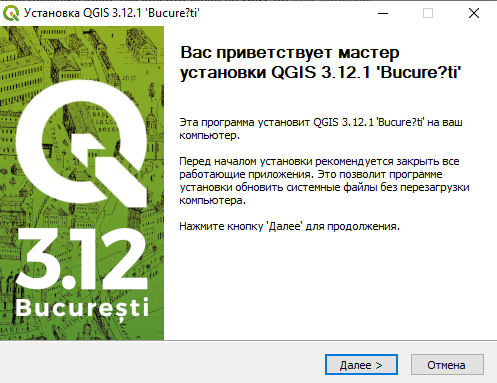
\includegraphics{images/installation_instruction_win/win01.png}

Нажмите «Далее», чтобы перейти на следующий шаг

На следующем шаге будет показано лицензионное соглашение QGIS и другого программного обеспечения, входящего в пакет поставки.

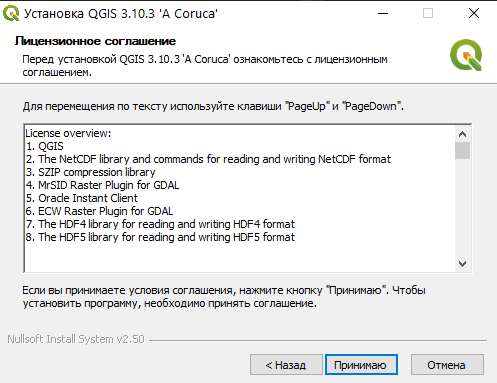
\includegraphics{images/installation_instruction_win/win02.png}

Нажмите «Принимаю».

На следующем шаге выберите папку для установки. По возможности используйте расположение, предлагаемое по умолчанию.

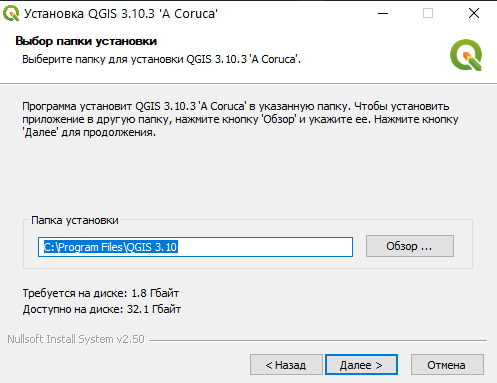
\includegraphics{images/installation_instruction_win/win03.png}

На следующем шаге предлагается выбрать дополнительные компоненты для установки. Снимите все флажки, кроме QGIS, и нажмите «Установить»

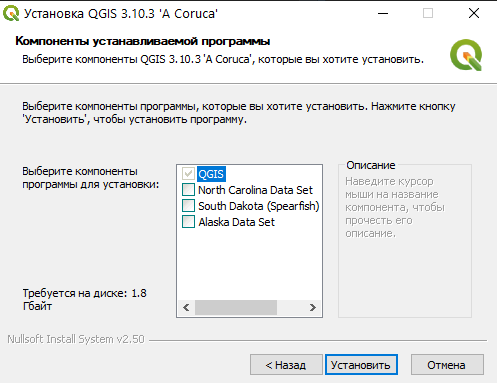
\includegraphics{images/installation_instruction_win/win04.png}

После окончания установки ярлыки QGIS будут добавлены в меню ``Пуск'' и в отдельную папку QGIS на рабочем столе.

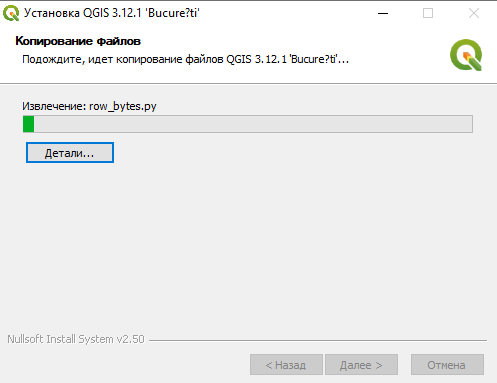
\includegraphics{images/installation_instruction_win/win05.png}

\hypertarget{macos}{%
\section*{macOS}\label{macos}}
\addcontentsline{toc}{section}{macOS}

Пользователи mac OS: используйте альтернативную сборку версии \href{https://www.kyngchaos.com/files/software/qgis/QGIS-macOS-3.4.12-1.dmg}{3.4.12}

Пользователи Linux: воспользуйтесь инструкциями по \href{https://qgis.org/ru/site/forusers/alldownloads.html\#linux}{этой ссылке}.

Дополнительную информацию по установке можно найти на \url{https://qgis.org/ru/site/forusers/download.html}.

\hypertarget{part-ux43eux441ux43dux43eux432ux44b-ux440ux430ux431ux43eux442ux44b-ux441-qgis}{%
\part{Основы работы с QGIS}\label{part-ux43eux441ux43dux43eux432ux44b-ux440ux430ux431ux43eux442ux44b-ux441-qgis}}

\hypertarget{map-design-general}{%
\chapter{Создание общегеографической карты}\label{map-design-general}}

\href{https://1drv.ms/u/s!AmtmZDq3JgxHgZUGIl2IXikh_JmrhA?e=NdRmIe}{Архив с данными и файлом отчёта}

\hypertarget{map-design-general-intro}{%
\section{Введение}\label{map-design-general-intro}}

\textbf{Цель задания} --- знакомство с моделями пространственных объектов и базой пространственных данных. Визуализация данных на карте. Оформление легенды и компоновки карты.

\textbf{Необходимая теоретическая подготовка:} модели пространственных данных, модели пространственных объектов, базы пространственных объектов, картографические проекции.

\textbf{Необходимая практическая подготовка:} практическая подготовка не требуется.

\textbf{Исходные данные:} база географических данных на территорию Кавказских гор, собранная из нескольких источников.

\textbf{Ожидаемый результат:} общегеографическая карта гор Кавказа и прилегающих территорий масштаба 1:4 500 000.

\hypertarget{map-design-general-checklist}{%
\subsection{Контольный лист}\label{map-design-general-checklist}}

\begin{itemize}
\tightlist
\item
  Добавить на карту источники пространственных данных и настроить их оформление
\item
  Настроить подписи объектов
\item
  Создать компоновку карты и легенду
\item
  Экспортировать результат в графический файл
\end{itemize}

\hypertarget{map-design-general-begin}{%
\section{Начало работы}\label{map-design-general-begin}}

\protect\hyperlink{map-design-general}{В начало упражнения ⇡}

\begin{enumerate}
\def\labelenumi{\arabic{enumi}.}
\item
  Скачайте архив с исходными данными для упражнения и распакуйте его в свою рабочую директорию.
\item
  Запустите \textbf{QGIS}. Для запуска воспользуйтесь иконкой с названием \textbf{\texttt{QGIS\ Desktop\ {[}...{]}\ with\ GRASS\ {[}...{]}}}.
\item
  Найдите \textbf{панель менеджера источников данных} 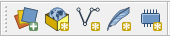
\includegraphics{images/Ex01/pic01.png} и откройте \textbf{Менеджер источников данных}.
\item
  В менеджере источников данных в режиме браузера найдите вашу рабочую директорию, а в ней --- каталог \texttt{Ex01\_GeneralMap\textbackslash{}raster\_data}. В этом каталоге отображается единственный источник данных --- \texttt{30n030e\_20101117\_gmted\_mea075.tif}. Иконка 
\includegraphics{images/Ex01/raster.png} и расширение \texttt{\textbackslash{}*.tif} (Tagged Image Tile Format) подсказывают вам, что этот источник представляет пространственные данные в растровой (регулярно-сеточной) модели.

  \begin{quote}
  Замечание 1: растр, с которым вы будете работать сейчас, сохранён в формате \href{https://www.opengeospatial.org/standards/geotiff}{GeoTIFF}. От «обычного» TIFF этот формат отличается тем, что сведения о пространственной привязке в GeoTIFF записываются непосредственно в файл с данными, в то время как «обычный» формат TIFF не поддерживает запись сведений о пространственной привязке, поэтому она хранится отдельно --- в \href{https://en.wikipedia.org/wiki/World_file}{world-файле}. В дальнейшем вы часто будете работать и с тем, и с другим способом хранения пространственных данных.
  \end{quote}

  \begin{quote}
  Замечание 2: файл \texttt{30n030e\_20101117\_gmted\_mea075.tif} является фрагментом («тайлом») глобальной цифровой модели рельефа (ЦМР) \href{https://www.usgs.gov/land-resources/eros/coastal-changes-and-impacts/gmted2010}{GMTED2010}. Этот источник часто используется для геоинформационного анализа и картографирования. Загрузить тайлы GMTED2010 можно через сервис \href{https://earthexplorer.usgs.gov/}{EarthExplorer} геологической службы США.
  \end{quote}
\item
  Дважды щёлкните левой кнопкой мыши на название файла \texttt{30n030e\_20101117\_gmted\_mea075.tif} в менеджере источников данных. В панель слоёв (по умолчанию слева) добавится слой с названием \texttt{30n030e\_20101117\_gmted\_mea075}.
\item
  Сохраните проект QGIS в папку с материалами упражнения (на том же иерархическом уровне, где находятся . Назовите его по шаблону \textless Ex01\_\%Фамилия\%\textgreater, где \%Фамилия\% --- ваша фамилия латинскими буквами.
\end{enumerate}

\textbf{Скриншот 1: Окно QGIS после загрузки набора данных.}

\begin{quote}
Примечание: файл проекта QGIS (*.qgs, *.qgz) и документ карты ArcGIS (*.mxd) отличаются от тех файлов, с которыми вы работали ранее. В этих файлах не хранятся пространственные данные, а только ссылки на них и настройки их отображения (включая порядок слоёв, символику и подписи). Если вы перемещаете файл проекта относительно источников данных, ссылки «теряются». Поэтому важно правильно организовать структуру ГИС-проекта. В рамках нашего упражнения мы разместили файл проекта в директории более высокого уровня по отношению к тем директориям, где лежат данные. Теперь, если мы переместим всю папку Ex01 вместе со всем её содержимым, относительные пути от файла проекта до файлов данных не изменятся, и проект сохранит работоспособность. Разумеется, такое простое решение не будет оптимальным для крупных организаций с разветвлённой структурой сетевых ресурсов, но для студенческих проектов оно, как правило, работает
\end{quote}

\hypertarget{map-design-general-projection}{%
\section{Настройка системы координат}\label{map-design-general-projection}}

\protect\hyperlink{map-design-general}{В начало упражнения ⇡}

В правом нижнем углу карты вы видите надпись 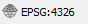
\includegraphics{images/Ex01/pic02.png}. Нажмите на эту надпись, чтобы открыть интерфейс выбора системы координат проекта.

В открывшемся окне вы видите более подробную информацию об используемой системе координат. Код \texttt{EPSG:4326} соответствует системе географических координат \textbf{WGS 84}. Термин «географическая система координат» (\emph{geographic coordinate systems}) в ГИС означает, что координаты объектов и линейные параметры растров хранятся в виде широты и долготы. Альтернативный подход --- проецированные системы координат (\emph{projected coordinate systems}), где плановые координаты измеряются в метрических единицах.

Система координат проекта была импортирована из первого (в нашем случае --- пока единственного) загруженного источника пространственных данных. Система координат WGS 84, как правило, не используется для картографирования, поэтому мы изменим систему координат проекта.

К настоящему моменту вы ещё не освоили курс «Математическая картография», в котором подробно разбираются вопросы разработки и выбора проекций для различных карт. Поэтому мы воспользуемся простым инструментом для выбора проекции --- \href{http://projectionwizard.org/}{Projection Wizard}.

\begin{enumerate}
\def\labelenumi{\arabic{enumi}.}
\item
  Перейдите на сайт \href{http://projectionwizard.org/}{Projection Wizard}. Настройте параметры территории и проекции следующим образом:

  Класс проекции по виду искажений: \textbf{равнопромежуточная}\\
  Охват территории картографирования: от 39° с.ш. до 46° с.ш., от 36° в.д. до 51° в.д.

  Вам будет предложено две проекции. \textbf{Нажмите на ссылку PROJ.4}, соответствующей \textbf{косой азимутальной} проекции. В верхней части экрана будет отображено всплывающее окно с параметрами выбранной проекции в формате \href{https://proj.org/usage/quickstart.html}{PROJ}.

  \begin{quote}
  формат PROJ, ранее известный как PROJ.4 --- один из трёх форматов описания системы координат, с которыми вы должны быть «на ты» по окончании курса геоинформатики. Другой формат --- коды \href{http://www.epsg-registry.org/}{EPSG} (удобный ресурс для поиска --- \href{https://epsg.io/}{epsg.io}). Эта международная база систем координат интегрирована почти во всё современное геоинформационное и окологеоинформационное ПО, включая QGIS. Третий вариант --- описание систем координат в формате Well-Known Text (WKT), применяемое в ArcGIS и некотором другом ПО.
  \end{quote}
\item
  Скопируйте строку PROJ в буфер обмена

  Также \textbf{вставьте скопированную строку в отчётный документ}
\item
  В QGIS откройте меню \textbf{Установки} --- \textbf{Пользовательские проекции\ldots{}}
\item
  Нажмите кнопку \textbf{Добавить новую проекцию}
\item
  В полях для ввода ниже введите название проекции: \emph{Azimuthal Equidistant (Caucasus)}, в поле «Параметры» скопируйте строку PROJ.
\item
  Нажмите \textbf{ОК}.

  Вы успешно добавили новую систему координат в пользовательский список. Теперь нужно применить её к проекту.
\item
  Откройте интерфейс выбора системы координат. Это можно сделать не только нажатием на элемент в правом нижнем углу, но и через меню \textbf{Проекты} --- \textbf{Свойства\ldots{}} (вкладка \textbf{Система координат}).
\item
  В открывшемся меню найдите в списке свою проекцию, выберите её и нажмите \textbf{ОК}.
\end{enumerate}

\textbf{Скриншот 2: Окно QGIS после изменения проекции}

Закройте интерфейс выбора системы координат и нажмите правой кнопкой на слой \texttt{30n030e\_20101117\_gmted\_mea075} в таблице слоёв. В контекстном меню выберите \textbf{Свойства\ldots{}} и в открывшемся окне перейдите на вкладку \textbf{Информация}. Вы видите, что проекция набора данных не изменилась. Просто QGIS умеет трансформировать наборы данных для отображения их в целевой проекции. Это называется «перепроецирование на лету́».

\hypertarget{map-design-general-navigation}{%
\section{Навигация по карте}\label{map-design-general-navigation}}

\protect\hyperlink{map-design-general}{В начало упражнения ⇡}

После изменения проекции центр карты сместился таким образом, что загруженный растр перестанет помещаться во фрейм карты. Нам в любом случае необходимо увеличить масштаб и переместить изображение, чтобы иметь возможность рассмотреть территорию картографирования более детально. Воспользуемся этим как поводом для освоения инструментов панели инструментов перемещения по карте:\\
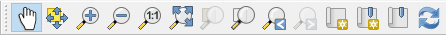
\includegraphics{images/Ex01/NavigationPanel.png}

Изучите функционал инструментов перемещения по карте. Некоторые из них могут быть задействованы независимо. Например, масштабирование выполняется прокруткой колеса мыши, а перемещение по карте --- движением мыши с зажатой средней кнопкой.

Когда освоитесь с функциями перемещения по карте, установите масштаб карты равным 1:5 000 000. Это можно сделать в элементе «Масштаб» в нижней панели QGIS. После этого переместите изображение таким образом, чтобы Кавказские горы простирались из северо-западного угла к юго-восточному.

\hypertarget{map-design-general-relief}{%
\section{Оформление рельефа}\label{map-design-general-relief}}

\protect\hyperlink{map-design-general}{В начало упражнения ⇡}

Изображение рельефа, которые вы видите, представляет собой так называемую аналитическую отмывку по высоте. Для аналитической отмывки используется шкала оттенков серого, применяемая по умолчанию. Мы будем использовать аналитическую отмывку по высоте вместе со светотеневой отмывкой.

\begin{enumerate}
\def\labelenumi{\arabic{enumi}.}
\item
  Откройте свойства слоя \texttt{30n030e\_20101117\_gmted\_mea075} и перейдите на вкладку \textbf{Стиль}.
\item
  Измените тип представления с \emph{Одноканальное серое} на \emph{Одноканальное псевдоцветное}.
\item
  Установите минимальное значение равным \emph{0}, а максимальное значение --- \emph{4000}.
\item
  В строке выбора градиента нажмите правой кнопкой на шкалу и в открывшемся контекстном меню выберите опцию \textbf{Создать новый градиент}
\item
  В появившемся всплывающем окне в ниспадающем списке выберите тип градиента \emph{Catalog: cpt-city} (\href{http://soliton.vm.bytemark.co.uk/pub/cpt-city/}{подробнее о cpt-city})
\item
  В открывшемся каталоге в разделе \emph{Topography} выберите градиент \emph{c3t3} и нажмите \textbf{OK}
\item
  После нажатия OK были закрыты все окна, кроме окна свойств слоя \texttt{30n030e\_20101117\_gmted\_mea075}. Нажмите \textbf{OK}, чтобы применить изменения символики и закрыть окно.

  Вы успешно применили аналитическую отмывку по высоте к цифровой модели рельефа. Но для красочного, визуально привлекательного изображения этого недостаточно. Помимо аналитической отмывки по высоте, мы создадим светотеневую отмывку.
\item
  Щёлкните правой кнопкой мыши по слою \texttt{30n030e\_20101117\_gmted\_mea075} в таблице слоёв и в контекстном меню нажмите \textbf{Дублировать слой}.

  Дубликат слоя будет помещён в таблице слоёв ниже исходного слоя, выключен, а к его имени будет приписано ``копия''.

  \emph{\textbf{Обратите внимание, что оба слоя используют один и тот же источник данных.} Вы можете сделать сколько угодно слоёв с разными настройками визуализации на базе одного и того же набора пространственных данных. Но если вы измените используемый набор пространственных данных, это повлечёт за собой автоматическое изменение вида слоёв (но не настроек их визуализации).}
\item
  Используя контекстное меню или окно свойств слоя, переименуйте оба слоя. Нижний слой назовите \emph{Аналитическая отмывка по высоте}, верхний --- \emph{Светотеневая отмывка}.

  \emph{Названия слоёв никак не затрагивают источник пространственных данных. До тех пор, пока вам не приходится работать со слоями с помощью скриптов на языке Python, вы можете никак не ограничивать себя в названиях.}
\item
  Включите отображение нижнего слоя.
\item
  Откройте свойства слоя «Светотеневая отмывка», перейдите на вкладку «Стиль».
\item
  Измените способ визуализации на \emph{Теневой рельеф} и нажмите \textbf{Применить}. При этом изменения будут применены, но окно свойств не закроется.

  На заднем плане вы видите изменения, произошедшие с вашим слоем. Во-первых, изображение светотеневой отмывки полностью закрыло изображение аналитической отмывки по высоте. Эту проблему можно решить, включив настройки прозрачности для слоя. Во-вторых, сама светотеневая отмывка выглядит очень тёмной. Это связано с несовпадением единиц измерения «по горизонтали» и «по вертикали» в исходном наборе данных. В нашем случае эту проблему можно решить двумя путями: трансформировать слой в проецированную систему координат или применить коэффициент масштабирования по вертикали (\emph{Z-factor}). Мы пойдём вторым путём и будем изменять значение коэффициента масштабирования.

  Коэффициент масштабирования представляет собой переводной коэффициент из «вертикальных» единиц измерения в «горизонтальные». Поскольку «горизонтальные» единицы в нашем случае --- градусы, и поскольку протяжённость одного градуса по долготе и по широте не совпадает, с его вычислением могут возникнуть сложности.

  \textbf{Вопрос*: Рассчитайте коэффициент масштабирования по отношению к 1° долготы и 1° широты (на широте параллели касания проекции), ответ запишите в виде обыкновенной дроби.}

  Чтобы не тратить время на точные расчёты, мы воспользуемся значением \emph{0,000012}
\item
  Помимо переводного коэффициента между единицами измерения, нам нужно дополнительно масштабировать высоты по вертикали, чтобы отмывка выглядела более «рельефно». В разных случаях применяется дополнительный множитель в диапазоне от 1,5 до 10, мы воспользуемся коэффициентом \emph{5}.
\item
  Перемножьте оба коэффициента и введите полученное значение в качестве Z-фактора слоя.
\item
  Перейдите на вкладку \textbf{Прозрачность} и установите коэффициент непрозрачности для слоя равным 50 \%. Примените изменения, закройте окно свойств слоя и сохраните проект.
\end{enumerate}

\textbf{Скриншот 3: полученное изображение рельефа}

\emph{Примечание для картографов: настройки визуализации рельефа, которые вы применили в этом упражнении, подобраны «на скорую руку», без предварительного анализа распределения высот картографируемой территории и выбора оптимальной шкалы. Эти вопросы подробно освещаются в курсах «Оформление карт» и «Общегеографическое картографирование».}

\hypertarget{map-design-general-vector}{%
\section{Добавление векторных наборов данных}\label{map-design-general-vector}}

\protect\hyperlink{map-design-general}{В начало упражнения ⇡}

Вновь откройте менеджер источников данных в виде браузера и перейдите в директорию «Размещение по умолчанию для проекта». Раскройте папку \emph{vector\_data}.

\begin{quote}
Размещение по умолчанию для проекта --- это директория, в которую был сохранён проект QGIS (*.qgz).
\end{quote}

\begin{figure}
\centering
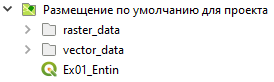
\includegraphics{images/Ex01/DefaultLocation.png}
\caption{Default location}
\end{figure}

Вы видите несколько источников данных, обозначенных символом 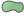
\includegraphics{images/Ex01/polygon.png}. Это векторные наборы данных, представленные в формате \href{https://desktop.arcgis.com/ru/arcmap/latest/manage-data/shapefiles/what-is-a-shapefile.htm}{шейп-файлов}.

Теперь откройте эту же директорию через Проводник Windows (или любой другой файловый менеджер). Сравните количество файлов в Проводнике с количеством доступных источников данных в браузере QGIS

\begin{quote}
Шейп-файлы были базовым форматом ГИС-пакета ArcView и за счёт этого получили очень широкое распространение. Шейп-файлы не такие функциональные, как базы геоданных ESRI (современный базовый формат для продуктов линейки ArcGIS) или GeoPackage, но тем не менее их продолжают активно использовать.\\
Многие особенности шейп-файлов обусловлены спецификой и возможностями компьютеров начала 90-х гг. В частности, геометрия набора данных хранится отдельно (в файле \texttt{.shp}), семантика --- отдельно (в формате dBASE, \texttt{.dbf}), а для связи между ними используется индекс-файл (\texttt{.shx}). Эти три файла --- обязательные компоненты шейп-файла. Помимо них, отдельно могут быть записаны сведения о проекции (\texttt{.prj}), кодировке (\texttt{.cpg}) и многое другое.\\
При копировании шейп-файла через Проводник необходимо копировать все файлы с одинаковым именем целиком.
\end{quote}

\begin{enumerate}
\def\labelenumi{\arabic{enumi}.}
\item
  Добавьте на карту наборы данных об объектах гидрографии (\texttt{hydrography-polyline.shp}, \texttt{hydrography-polygon.shp}). В таблице слоёв разместите линии над полигонами. Переименуйте слои в «Водотоки» и «Водоёмы» соответственно.

  \begin{quote}
  Все векторные наборы данных для этого упражнения созданы на основе \href{http://www.vsegei.com/ru/info/topo/}{цифровых географических основ ВСЕГЕИ}. Это один из немногих общедоступных источников пространственных данных общегеографического содержания на территорию нашей страны и ближнего зарубежья.
  \end{quote}
\item
  Настройте символику для добавленных векторных наборов данных. Также, как и для растров, настройки символики векторных данных помещаются в свойствах слоя, на вкладке «Стиль».

  Для полигонов гидрографии установите стандартный стиль \emph{topo water} из библиотеки QGIS.

  Для линейных объектов используйте стандартный стиль \emph{simple blue line}, но уменьшите толщину линии до 0,26 мм

  \begin{quote}
  Если приглядеться, то можно увидеть, что знак контура береговой линии и знаки линейных объектов гидрографии на суше не совпадают. Можно изменить цвет и толщину обводки для полигонов объектов гидрографии, сделав их такими же, как у рек и каналов.
  \end{quote}
\item
  Добавьте к карте железные дороги и автодороги. Переименуйте слои и изобразите их линиями толщиной 0,26 мм. Для автодорог используйте красный цвет, для железных дорог --- тёмно-серый (20 \% светлоты).
\end{enumerate}

\hypertarget{map-design-general-attributes}{%
\section{Использование атрибутов объектов при визуализации}\label{map-design-general-attributes}}

\protect\hyperlink{map-design-general}{В начало упражнения ⇡}

До этого момента мы работали только визуальным представлением слоя и никак не касались семантической составляющей. На следующем шаге вы будете использовать разные значки для различных типов объектов в одном слое.

\begin{enumerate}
\def\labelenumi{\arabic{enumi}.}
\item
  Добавьте к карте набор данных \texttt{adm\_line}, переместите добавленный слой ниже всех линейных объектов и переименуйте его в «Границы».
\item
  Вызовите контекстное меню слоя «Границы» и выберите опцию «Открыть таблицу атрибутов». Откроется таблица атрибутов источника данных.

  \begin{figure}
  \centering
  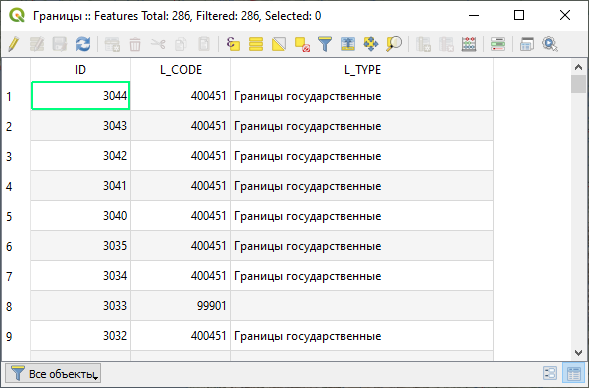
\includegraphics{images/Ex01/AttributeTable.png}
  \caption{Attribute Table}
  \end{figure}

  Таблица атрибутов --- это представление базы данных, связанной с набором пространственных объектов. База функционирует по общим правилам реляционной базы данных: каждый объект представляется одной «строкой», в каждом столбце (поле) одному объекту соответствует одно значение. Атрибуты играют важную роль в геоинформационных системах. На их основе происходит визуализация данных, также они участвуют в большинстве операций пространственного анализа. В этом упражнении вы используете атрибуты, чтобы присвоить различные стили объектам в одном слое.
\item
  Закройте таблицу атрибутов, откройте свойства слоя на вкладке «Стиль»
\item
  Измените тип визуализации с \emph{Обычный знак} на \emph{Уникальные значения}. Эта настройка позволяет присваивать объектам различные стили в соответствии со значениями определённого атрибута.
\item
  В выпадающем списке \textbf{Поле} выберите столбец, по которому будет происходить классификация, и нажмите кнопку \textbf{Классифицировать} внизу формы.

  В форму добавились три записи. Две из них представляют фактически имеющиеся значения атрибутов, третья --- «пустая» --- предназначена для визуализации всех остальных значений (которых фактически нет в таблице на настоящий момент, но которые могут появиться позже в результате редактирования)

  \begin{figure}
  \centering
  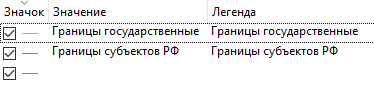
\includegraphics{images/Ex01/Classes.png}
  \caption{Classes}
  \end{figure}

  Возможности автоматической настройки визуализации у QGIS пока невелики по сравнению с ArcGIS или MapInfo. Например, сейчас нашим классам присвоены стили в виде линий, у которых совпадают все параметры, кроме цвета. По-другому QGIS (пока) не умеет .

  Наша задача --- создать разные условные знаки для разных типов границ
\item
  Дважды щёлкните на значке, соответствующем классу \emph{Границы государственные}. Откроется уже знакомый вам интерфейс настройки условных знаков. Обратите внимание на форму в левом верхнем углу: вы можете задать несколько слоёв для одного условного знака.

  \begin{quote}
  Разумеется, слои в таблице слоёв и слои условного знака --- это две не связанные между собой сущности
  \end{quote}
\item
  Создайте для государственных границ двухслойный знак. Нижний слой: линия серого цвета (75 \% светлоты) шириной 1 мм, с плоскими концами (чтобы концы линии не «свешивались» в воду). Верхний слой: линия тёмно-серого цвета (светлота 20 \%) толщиной 0,26 мм, штрихпунктирная, с плоскими концами.
\item
  Создайте аналогичный знак для границ субъектов РФ. Нижний слой: линия серого цвета (75 \% светлоты) шириной 0,8 мм, с плоскими концами. Верхний слой: линия тёмно-серого цвета (светлота 20 \%) толщиной 0,26 мм, штриховая, с плоскими концами.
\item
  Для прочих границ используйте однослойный условный знак: пунктирная линия тёмно-серого цвета
\end{enumerate}

Вы успешно настроили разные условные знаки для различных типов объектов в слое. Сохраните проект.

\textbf{Далее мы не будем напоминать вам о необходимости сохранять проект карты. Делайте это самостоятельно.}

\hypertarget{map-design-general-labels}{%
\section{Подписи}\label{map-design-general-labels}}

\protect\hyperlink{map-design-general}{В начало упражнения ⇡}

\begin{enumerate}
\def\labelenumi{\arabic{enumi}.}
\item
  Добавьте на карту набор данных \texttt{elevation\_points.shp}, расположите слой на самом верху списка и переименуйте его в «Вершины». Настройте отображение единым знаком в виде чёрного треугольника, аналогично тому, как высочайшие отметки показываются в школьных атласах.
\item
  Откройте таблицу атрибутов слоя. Какие поля можно использовать для подписей?

  \begin{quote}
  На общегеографических картах обычно приводятся высоты и названия горных вершин. В этом упражнении мы ограничимся названиями.
  \end{quote}
\item
  Закройте таблицу атрибутов и откройте свойства слоя. Перейдите на вкладку «Подписи». Переключите режим подписей на \emph{Single labels} («Подписывать объекты значением атрибута»). В открывшемся меню в выпадающем списке «Подписывать значениями» выберите поле \texttt{Name} --- тексты подписей будут «считываться» из него.
\item
  В поле \textbf{Text sample} отображается пример подписи с теми настройками, которые заданы по умолчанию. Если вы будете менять настройки подписей (шрифт, форматирование, «гало» и др.), этот приме будет меняться. Сейчас мы последовательно пройдём по вкладкам настройки подписей, исправив необходимые параметры.

  На вкладке \emph{Текст} установите гарнитуру («шрифт») Times New Roman, начертание («стиль») полужирный курсив, кегль («размер») 8.

  На вкладке \emph{Тень} включите опцию «Рисовать падающую тень». Это повысит читаемость подписей на карте.

  \begin{quote}
  Также с целью повышения читаемости подписей можно использовать обводку («Буфер») и фон (англ. \emph{Background}, неправильно переведён как «История»).
  \end{quote}

  На вкладке \emph{Размещение} выберите опцию «Картографическое», расстояние 0,1 мм от границ символа (\emph{from symbol bounds})

  Примените настройки подписей и закройте свойства слоя
\item
  В каталоге \texttt{vector\_data} остался незадействованный слой --- \texttt{population\_points}. Добавьте его в проект? переименуйте и самостоятельно настройте условные знаки и подписи. Используйте параметр \emph{уникальные значения} для того, чтобы отобразить города с разной численностью населения разными условными знаками.
\end{enumerate}

\textbf{Скриншот 4: окно QGIS после завершения настройки символов}

\hypertarget{map-design-general-layout}{%
\section{Настройка компоновки карты}\label{map-design-general-layout}}

\protect\hyperlink{map-design-general}{В начало упражнения ⇡}

Изображение, которое вы видите во фрейме данных, можно экспортировать «как есть» (с помощью опции «Проекты» --- «Импорт/экспорт» --- «Экспортировать карту как изображение\ldots»). Однако для картографических целей мы, как правило, формируем \textbf{компоновку карты} --- размещаем картографическое изображение на листе, добавляем название, легенду, масштабную линейку и элементы зарамочного оформления.

Сейчас мы создадим макет компоновки с расчётом на то, что итоговая карта будет вставлена в отчёт.

\begin{enumerate}
\def\labelenumi{\arabic{enumi}.}
\item
  Создайте новый макет компоновки («Проект» --- «Создать Макет\ldots») или \texttt{Ctrl+P}.
\item
  Введите название макета на своё усмотрение.

  После ввода названия откроется окно компоновки (\emph{Layout})\\
  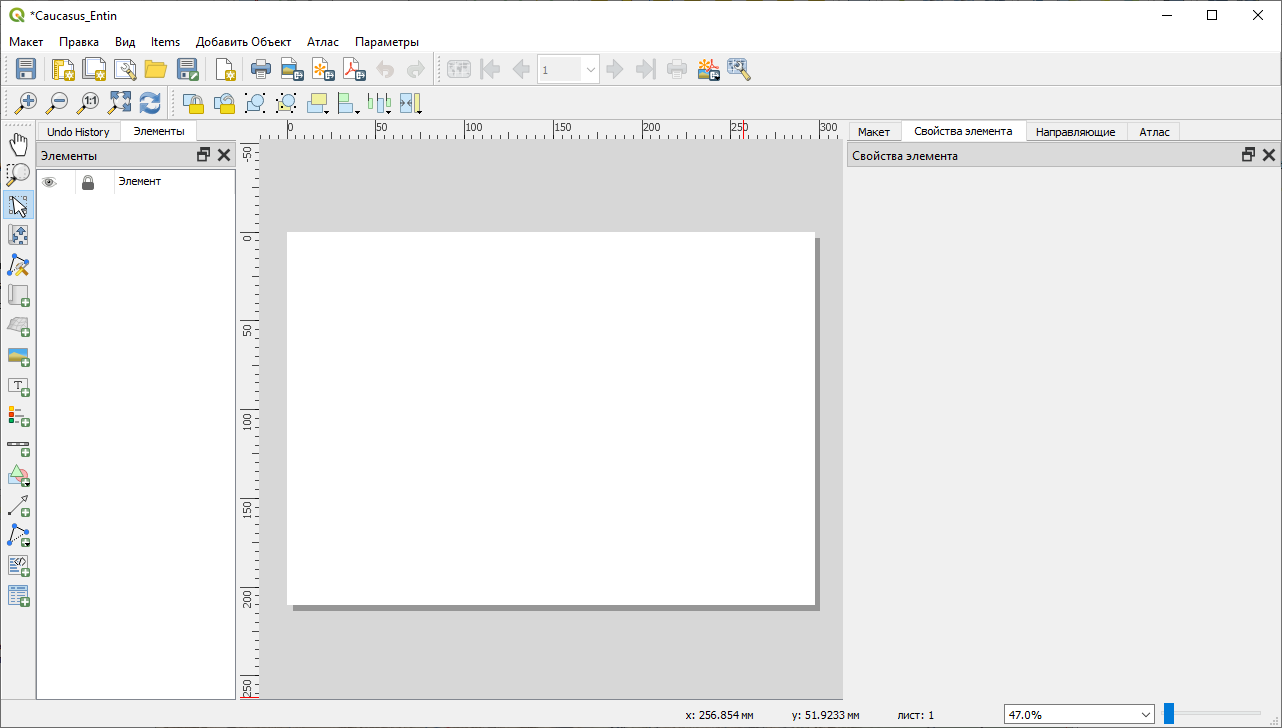
\includegraphics{images/Ex01/Layout.png}
\item
  Добавьте на лист картографическое изображение. Для этого используется инструмен «Добавить карту» из панели инструментов. Выберите инструмент и «растяните» прямоугольник карты на листе.
\item
  После добавления элемента откроется панель его свойств. Изучите настройки, доступные в этой панели, а затем установите для карты знаменатель масштаба \emph{4 000 000} и размеры 237 × 130 мм. В том же разделе, где устанавливаются размеры элемента, задайте для элемента карты положение по X = 30 мм и положение по Y = 30 мм.

  \begin{quote}
  Положение элемента на листе отсчитывается от верхнего левого угла листа до точки привязки элемента.
  \end{quote}
\item
  Добавьте к карте градусную сетку. Для этого в свойствах элемента найдите раздел «Сетки», нажмите на кнопку \emph{Добавить новую сетку}, а затем \emph{Modify Grid}. Откроется меню настройки сетки. Задайте для сетки проекцию WGS84, интервал по долготе --- 4°, интервал по широте --- 2°. Также уменьшите толщину линий сетки до 0,1 мм. Для этого щёлкните левой кнокой мыши по элементу \emph{Стиль линии}, откроется уже привычный вам интерфейс настройки условного знака. Вернуться обратно к настройкам сетки можно, нажав на кнопку «Назад» в левом верхнем углу интерфейса.
\item
  Добавьте рамку сетки в виде простой линии и включите отображение подписей координатной сетки. Настройте отображение подписей так, чтобы широта подписывалась только вдоль западной и восточной рамки, а долгота --- только вдоль северной и южной. Используйте формат координат \emph{Десятичные с окончанием} и нулевое число знаков после запятой (этот параметр в QGIS называется «Точность координат»)
\item
  Вернитесь к макету и передвиньте картографическое изображение внутри элемента таким образом, чтобы вместилась вся основная часть Главного Кавказского хребта. Можно ориентироваться на города: в северо-западном углу карты должен отображаться Краснодар, в юго-восточном --- Баку.

  Для перемещения карты внутри фрейма используется инструмент «Перемещение содержимого элемента»
\item
  Добавьте на лист \textbf{название карты}. Для этого \textbf{вставьте новую надпись} и разместите её над элементом карты. Введите название карты «Кавказские горы», используйте выключку по середине, настройте параметры шрифта на своё усмотрение.
\item
  Добавьте на лист \textbf{масштабную линейку}. Переместите линейку в юго-западный угол карты, установите для неё отображение фона и границы, исправьте обозначение единиц измерения. Уменьшите высоту линейки, кегль шрифта и отступы подписей, чтобы линейка смотрелась более компактно.
\item
  Добавьте на лист \textbf{легенду}. Легенда будет собрана автоматически на основе тех настроек визуализации, которые применены для слоёв карты.
\item
  Отредактируйте легенду. Для этого сначала выключите автообновление (\emph{Auto update}) элементов легенды, чтобы сделать список элементов доступным для редактирования. Удалите из легенды те условные знаки, которые не встречаются на карте, и переименуйте неинформативные или пустые подписи.
\item
  Добавьте обводку для элемента легенды и разместите элемент в северо-восточном углу карты.
\item
  Добавьте ещё один текстовый элемент и впишите в него сведения об авторстве.
\item
  Экспортируйте получившуюся карту в изображение формата PNG («Макет» --- «Экспорт в изображение\ldots» или специальная кнопка на главной панели инструментов макета).
\end{enumerate}

\hypertarget{map-design-quaternary}{%
\chapter{Создание карты четвертичных отложений}\label{map-design-quaternary}}

\href{https://1drv.ms/u/s!AmtmZDq3JgxHgZUFCgDwGfEvocDIrw?e=LZbP6h}{Архив с данными и файлом отчёта}

\hypertarget{map-design-quaternary-intro}{%
\section{Введение}\label{map-design-quaternary-intro}}

\textbf{Цель задания} --- закрепление навыков загрузки и визуализации данных в QGIS.

\textbf{Необходимая теоретическая подготовка:} модели пространственных данных, модели пространственных объектов, базы пространственных объектов, картографические проекции.

\textbf{Необходимая практическая подготовка:} в объёме упражнения 1.

\textbf{Исходные данные:} база геоданных ESRI на территорию Сатинского учебного полигона, Калужская область.

\textbf{Ожидаемый результат:} карта четвертичных отложений Сатинского полигона М 1:30 000

\hypertarget{map-design-quaternary-checklist}{%
\subsection{Контольный лист}\label{map-design-quaternary-checklist}}

\begin{itemize}
\tightlist
\item
  Добавить на карту источники пространственных данных
\item
  Импортировать символику
\item
  Настроить подписи объектов
\item
  Создать набор пространственных данных из текстового файла
\item
  Создать компоновку карты и легенду
\item
  Экспортировать результат в графический файл
\end{itemize}

\hypertarget{map-design-quaternary-begin}{%
\section{Начало работы}\label{map-design-quaternary-begin}}

\protect\hyperlink{map-design-quaternary}{В начало упражнения ⇡}

\begin{enumerate}
\def\labelenumi{\arabic{enumi}.}
\item
  Скачайте архив с исходными данными для упражнения и распакуйте его в свою рабочую директорию.

  В вашей рабочей директории появилась «папка» \texttt{Satino.gdb}. Зайдя в неё с помощью проводника или Finder'a, вы увидите множество файлов с различными расширениями (\emph{.spx, }.gdbtable, *.gdbtablx и др.). Ничего не редактируйте в этой «папке».
\item
  Запустите \textbf{QGIS} и сразу сохраните проект в своей рабочей директории, на одном иерархическом уровне с \texttt{Satino.gdb}. Назовите его по шаблону \texttt{Ex02\_\%Фамилия.qgz\%}.

  \begin{quote}
  Примечание: не забывайте периодически сохранять проект QGIS!
  \end{quote}
\item
  Откройте Менеджер источников данных и разверните содержимое базы \texttt{Satino.gdb}

  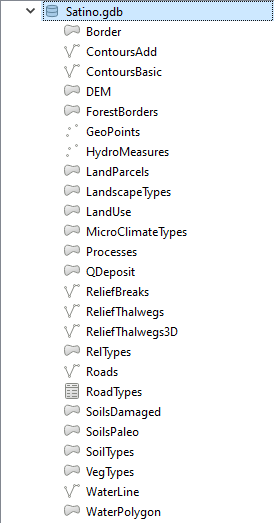
\includegraphics{images/Ex02/ArcGIS_GDB.png}

  Вы видите список наборов пространственных данных, хранящихся в базе \texttt{Satino.gdb}. Это векторные наборы различной геометрии (точечной, линейной и полигональной).

  \begin{quote}
  База геоданных ESRI (*.gdb) --- основной формат, используемый линейкой программных продуктов ArcGIS. В базах геоданных могут храниться как векторные, так и растровые данные. Кроме того, базы геоданных поддерживают специальные возможности (подтипы, доменты) и структуры данных (топологические и сетевые наборы).
  \end{quote}

  \begin{quote}
  QGIS способен получать доступ к базам геоданных ESRI в режиме чтения, но не в режиме редактирования. И даже эти возможности ограничены: QGIS «видит» векторные наборы пространственных данных, но «не считывает» структуру базы (классы и наборы пространственных объектов), растровые наборы, топологию и другие элементы, специфические для ArcGIS. В частности, набор DEM, который отображается в браузере как векторный полигональный набор данных, на самом деле является растровым набором.
  \end{quote}
\end{enumerate}

\hypertarget{map-design-quaternary-data}{%
\section{Добавление данных в проект}\label{map-design-quaternary-data}}

\protect\hyperlink{map-design-quaternary}{В начало упражнения ⇡}

\begin{enumerate}
\def\labelenumi{\arabic{enumi}.}
\item
  Добавьте на карту наборы \texttt{WaterLine}, \texttt{WaterPolygon} и \texttt{QDeposit}.

  \textbf{Вопрос 1:} какая система координат присвоена для каждого набора данных? Какая проекция используется для этой системы координат? К какому виду относится эта проекция по характеру искажений? Для чего она применяется?\\
  \textbf{Вопрос 2:} какая система координат присвоена проекту QGIS после добавления набора данных?
\item
  Настройте визуализацию слоёв \texttt{WaterLine} и \texttt{WaterPolygon}, используя условные знаки из библиотеки QGIS. Окно QGIS должно принять вид, аналогичный рисунку ниже:

  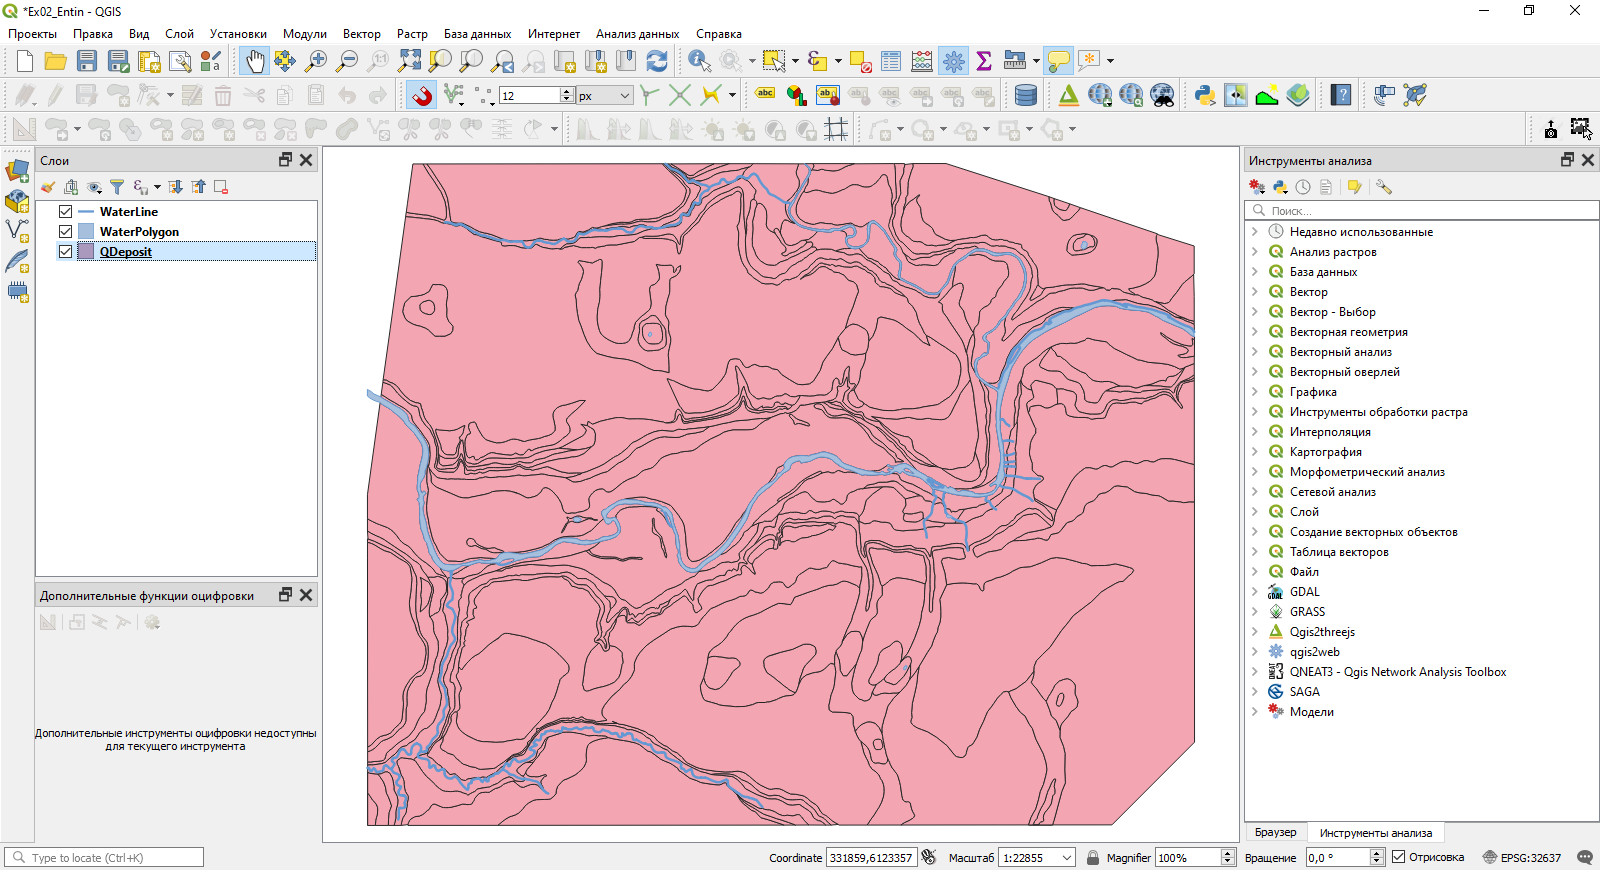
\includegraphics{images/Ex02/Example1.png}
\item
  Откройте таблицу атрибутов слоя \texttt{QDeposit} и изучите её.

  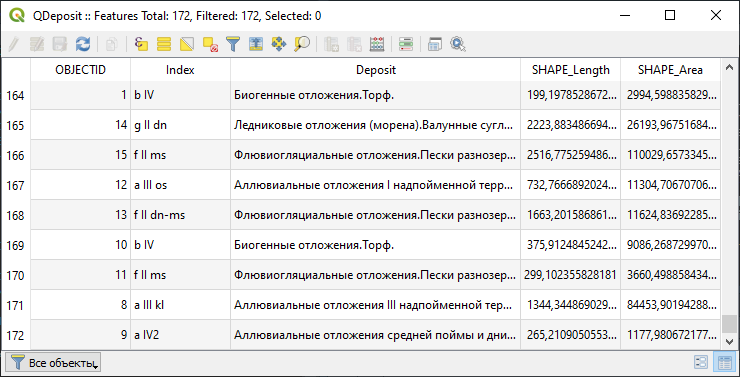
\includegraphics{images/Ex02/AttributeTable.png}

  Вы видите индексы и текстовые описания четвертичных отложений. Далее вы визуализируете слой QDeposit таким образом, что каждому типу отложений (\texttt{Deposit}) будет сопоставлен уникальный условный знак.
\end{enumerate}

\hypertarget{map-design-quaternary-classification}{%
\section{Применение готового стиля к слою}\label{map-design-quaternary-classification}}

\protect\hyperlink{map-design-quaternary}{В начало упражнения ⇡}

\begin{enumerate}
\def\labelenumi{\arabic{enumi}.}
\item
  Откройте свойства слоя \texttt{QDeposit}.
\item
  На вкладке «Стиль» измените тип отображения на \emph{Уникальные значения} и настройте классификацию по полю \texttt{Index} c использованием случайных цветов (\emph{Random colors}). Закройте свойства слоя и оцените результат.

  \textbf{Скриншот 1:} результат классификации --- отображение каждого типа отложений уникальным цветом.
\item
  Изображение стало более «пёстрым», но не стало более читаемым. Человеческому глазу трудно распознать два десятка уникальных оттенков цвета. Кроме того, исходя из географической логики, родственным категориям должны быть присвоены схожие цвета.

  Разработка цветовых решений для сложных, комплексных карт является отдельной научной задачей. В этом упражнении вы будете использовать готовые наборы стилей.
\item
  В левом нижнем углу вкладки «Стиль» найдите кнопку «Стиль». Нажмите на неё и выберите опцию «Загрузить стиль». В открывшемся окне в строчке «Файл» найдите стилевой файл \texttt{QDeposit.qml}. Загрузите из этого файла всю доступную символику.

  \begin{quote}
  QGIS, как и другое геоинформационное ПО, позволяет сохранять настройки отображения слоя в отдельный стилевой файл. Поддерживаются два формата: QGIS Layer Style File (\emph{.qml) и Styled Layer Descriptor (}.sld). В проприетарном ПО (ArcGIS, MapInfo) используются другие форматы описания стилей. Как правило, они несовместимы друг с другом.
  \end{quote}

  \textbf{Скриншот 2:} изображение готового слоя после импорта символики
\item
  Изучите условные знаки, применённые для слоя, и ответьте на вопросы:

  \textbf{Вопрос 3}: чем отличается условный знак, применённый для биогенных отложений, от всех прочих условных знаков? Каким образом это осуществлено?

  \textbf{Вопрос 4}: как соотносятся записи в таблице атрибутов (поле Deposit) и записи в поле «Легенда» в настройках стиля условных знаков?
\item
  Настройте подписи для слоя. Для подписывания используйте поле Index. Настройки подписей определите самостоятельно.
\end{enumerate}

\hypertarget{map-design-quaternary-csv}{%
\section{Создание набора пространственных данных из таблицы с координатами}\label{map-design-quaternary-csv}}

\protect\hyperlink{map-design-quaternary}{В начало упражнения ⇡}

\begin{enumerate}
\def\labelenumi{\arabic{enumi}.}
\item
  Найдите в проводнике файл \texttt{geol\_points.csv} и откройте его с помощью простого текстового редактора (Блокнот или аналогичный). Изучите содержимое файла.

  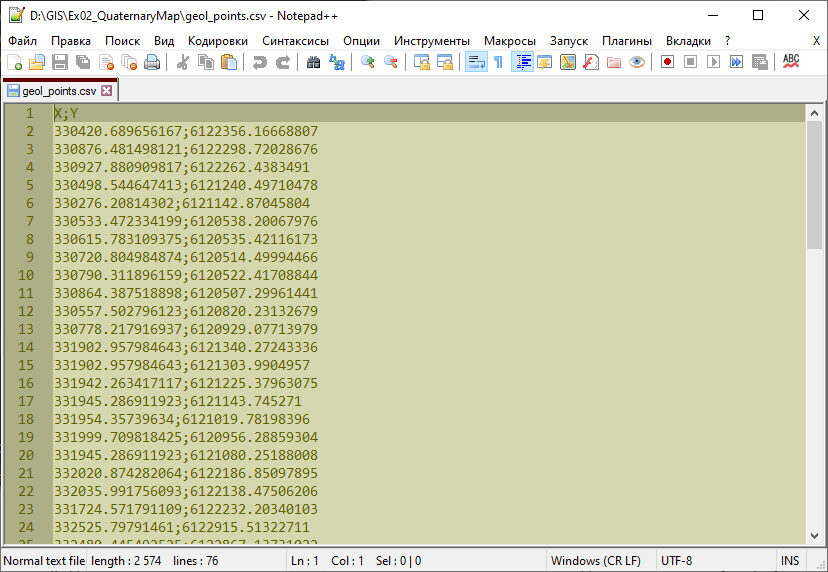
\includegraphics{images/Ex02/csv.png}

  \begin{quote}
  Comma-Separated Values (CSV) --- простой текстовый формат, предназначенный для хранения табличных данных. Каждая строка представляет строку таблицы, а ячейки, соответствующие столбцам, разделяются специальными символами. В качестве такого символа может быть использована запятая, точка с запятой, знак табуляции или сочетание из нескольких символов.
  \end{quote}

  В представленном файле вы видите два столбца --- X и Y. Это представление координат точек. Система координат, которая использовалась при создании файла, совпадает с системой координат вашего проекта. На следующих шагах вы загрузите эту таблицу в QGIS как набор пространственных данных.
\item
  Откройте панель менеджера источников данных и перейдите на вкладку \emph{Delimited Text}. Поскольку текстовый файл не содержит сведений, необходимых для корректного импорта и визуализации, мы будем настраивать параметры импорта вручную.
\item
  Нажмите значок с символом \texttt{...} справа от первого поля и в окне Проводника откройте файл \texttt{geol\_points.csv}. Не меняйте имя слоя и кодировку.

  \begin{quote}
  Примечание: в дальнейшем в вашей практике будут встречаться CSV-файлы, созданные в различных кодировках. В таких случаях нужно будет выбрать (или подобрать) правильную кодировку. Проверить себя можно по образцу загружаемой таблицы, который отображается в нижней части интерфейса загрузчика.
  \end{quote}
\item
  В первом блоке настроек («Формат файла») установите корректный разделитель столбцов.
\item
  Во втором блоке настроек («Настройки полей и записей») установите нужные параметры самостоятельно.
\item
  В третьем блоке настроек («Геометрия») определите, какие поля содержат координаты точек, и установите целевую систему координат --- такую же, как система координат проекта.
\item
  В блоке «Настройки слоя» не меняйте значения, определённые по умолчанию.
\item
  Проверьте себя, посмотрев блок «Примеры данных». Если настройки заданы правильно, в этом блоке будут корректно отображены первые 20 строк таблицы (не считая заголовков).

  \textbf{Скриншот 3:} Окно настроек импорта CSV-файла
\item
  Нажмите кнопку «Добавить», чтобы добавить слой на карту.
\item
  Настройте условные знаки для добавленного слоя. Отобразите все разрезы чёрными кругами диаметром 1,4 мм без обводки.
\end{enumerate}

\hypertarget{map-design-quaternary-final}{%
\section{Оформление карты}\label{map-design-quaternary-final}}

\protect\hyperlink{map-design-quaternary}{В начало упражнения ⇡}

\begin{enumerate}
\def\labelenumi{\arabic{enumi}.}
\setcounter{enumi}{6}
\item
  Создайте макет карты в портретной ориентировке и добавьте на него картографическое изображение.
\item
  Установите следующие параметры элемента карты: ширина 170 мм, высота 140 мм, масштаб картографического изображения 1:30 000.
\item
  Разместите элемент карты в верхней половине листа
\item
  Настройте сетку \textbf{прямоугольных} координат для карты в виде перекрестий.

  \begin{quote}
  \emph{Подсказка: используйте для сетки ту же систему координат, которая применена для проекта QGIS в целом}
  \end{quote}
\item
  Добавьте зарамочное оформление: название карты, легенду, масштабную линейку.
\item
  Экспортируйте карту в формат PNG и вставьте её в отчётный документ.

  \begin{quote}
  \emph{Подсказка: используйте опцию «Обрезать по содержимому», чтобы сохранить размеры изображения в отчётном документе}
  \end{quote}
\end{enumerate}

\hypertarget{map-ref-districts}{%
\chapter{Привязка и цифрование административной карты}\label{map-ref-districts}}

\href{https://1drv.ms/u/s!AmtmZDq3JgxHgZUEGskg6DlUfpKdug?e=n6tNQA}{Архив с данными и файлом отчёта}

\hypertarget{map-ref-districts-intro}{%
\section{Введение}\label{map-ref-districts-intro}}

\textbf{Цель задания} --- знакомство с привязкой, трансформированием и цифрованием геоизображений, элементами базовых технологий ГИС (оверлей, пространственные запросы).

\textbf{Необходимая теоретическая подготовка:} Системы координат и проекции карт, привязка геоизображений, трансформирование геоизображений, цифрование геоизображений. Методы трансформации: аффинное, проективное, полиномиальное, метод резинового листа (сплайны). Пространственные запросы, атрибутивные запросы, оверлей.

\textbf{Необходимая практическая подготовка:} Знание основных компонент интерфейса QGIS (менеджер источников данных, панель слоёв, фрейм карты, окно настройки компоновки). Добавление источников пространственных данных в проект. Настройка символики и подписей объектов. Создание макета, добавление карты и зарамочного оформления, экспорт макета.

\textbf{Исходные данные:} Cлои картографической основы OpenStreetMap, растровая карта избирательных округов г. Белгорода.

\textbf{Результат:} Набор пространственных данных с избирательными округами г. Белгорода и статистикой по застройке в пределах округов. Картодиаграммы по количеству домов и степени застроенности. Картографическое изображение.

\hypertarget{map-ref-economic-control}{%
\subsection{Контрольный лист}\label{map-ref-economic-control}}

\begin{itemize}
\tightlist
\item
  Привязать растровую карту к опорным данным
\item
  Создать класс избирательных округов путем цифрования растровой карты
\item
  Добавить номера районов в таблицу атрибутов
\item
  Определить (путем применения серии пространственных запросов) структуру застройки в каждом округе
\item
  Построить картодиаграммы по полученным значениям
\item
  Подготовить проект карты с компоновкой
\end{itemize}

\hypertarget{map-ref-districts-basemap}{%
\section{Добавление базовых данных}\label{map-ref-districts-basemap}}

\protect\hyperlink{map-ref-districts}{В начало упражнения ⇡}

\begin{enumerate}
\def\labelenumi{\arabic{enumi}.}
\item
  Скачайте архив и распакуйте его в свою рабочую директорию.
\item
  Создайте проект QGIS и сохраните его в распакованную папку (\emph{Ex05\_RefAdm}) в своей рабочей директории.
\item
  В менеджере источников данных найдите расположение проекта и разверните содержимое базы \texttt{belgorod.gpkg}.

  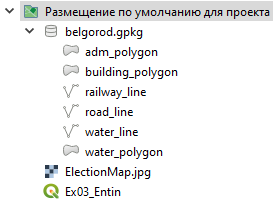
\includegraphics{images/Ex05/GeoPackage_structure.png}

  \begin{quote}
  Формат \href{http://www.geopackage.org/}{GeoPackage} был предложен в середине 2010-х как открытая \href{https://imgs.xkcd.com/comics/standards.png}{альтернатива существующим форматам} хранения пространственных данных: \href{http://switchfromshapefile.org/\#shapefileisbad}{шейп-файлу} и базам геоданных ESRI. GeoPackage представляет собой базу данных SQLite, внутри которой содержатся таблицы с данными и таблицы с метаданными. Такой подход аналогичен базе геоданных ESRI. Однако, в отличие от базы геоданных и от шейп-файлов, GeoPackage хранит всю необходимую информацию в одном файле (*.gpkg). Это позиционируется как одно из главных преимуществ формата.
  \end{quote}
\item
  Добавьте все наборы из базы \texttt{belgorod.gpkg} на карту.

  \begin{quote}
  \emph{Примечание: проще всего сделать это через менеджер источников данных. Другой вариант --- перетащить файл из окна системного файлового менеджера.}
  \end{quote}
\item
  Разместите слои в следующем порядке и настройте их символику:

  \begin{itemize}
  \tightlist
  \item
    \textbf{железные дороги:} тёмно-серые линии толщиной 0,4 мм;
  \item
    \textbf{автодороги:} светло-оранжевые линии толщиной 0,26 мм;
  \item
    \textbf{здания и сооружения:} заливка светло-серого цвета без обводки;
  \item
    \textbf{водоёмы:} используйте стиль \texttt{topo\ water};
  \item
    \textbf{водотоки:} синие линии толщиной 0,26 мм;
  \item
    \textbf{административные границы:} иcпользуйте стиль \texttt{outline\ red}.
  \end{itemize}

  Задайте слоям русскоязычные названия
\item
  Отобразите карту в охвате слоя границ.

  \textbf{Скриншот 1:} окно QGIS после завершения настройки символики

  \textbf{Вопрос 1:} какая система координат используется в проекте? Для чего обычно применяется эта система координат?
\end{enumerate}

\hypertarget{map-ref-districts-referencing}{%
\section{Привязка карты}\label{map-ref-districts-referencing}}

\protect\hyperlink{map-ref-districts}{В начало упражнения ⇡}

\begin{enumerate}
\def\labelenumi{\arabic{enumi}.}
\item
  Для привязки растров в QGIS имеется модуль «Привязка растров (GDAL)». Чтобы запустить его, выберите «Растр» --- «Привязка растров\ldots». Откроется окно модуля привязки.

  \begin{quote}
  Примечание: Если в меню «Растр» нет нужного пункта, следует зайти в меню «Модули» --- «Управление модулями\ldots» и в разделе «Установленные» включить модуль «Привязка растров (GDAL)». «Привязка растров» --- модуль, который входит в ядро QGIS, он обязательно устанавливается вместе с основной программой.
  \end{quote}
\item
  В окне привязки нажмите кнопку «Открыть растр» и откройте файл \texttt{ElectionMap.jpg}, который находится в вашей рабочей директории. При загрузке QGIS попросит вас указать систему координат для добавляемого растра. Выбирайте ту же систему координат, которая используется в проекте.
\item
  Расположите окно модуля привязки таким образом, чтобы оно не закрывало основной фрейм карты. Выключите панели инструментов QGIS, если они вам мешают.

  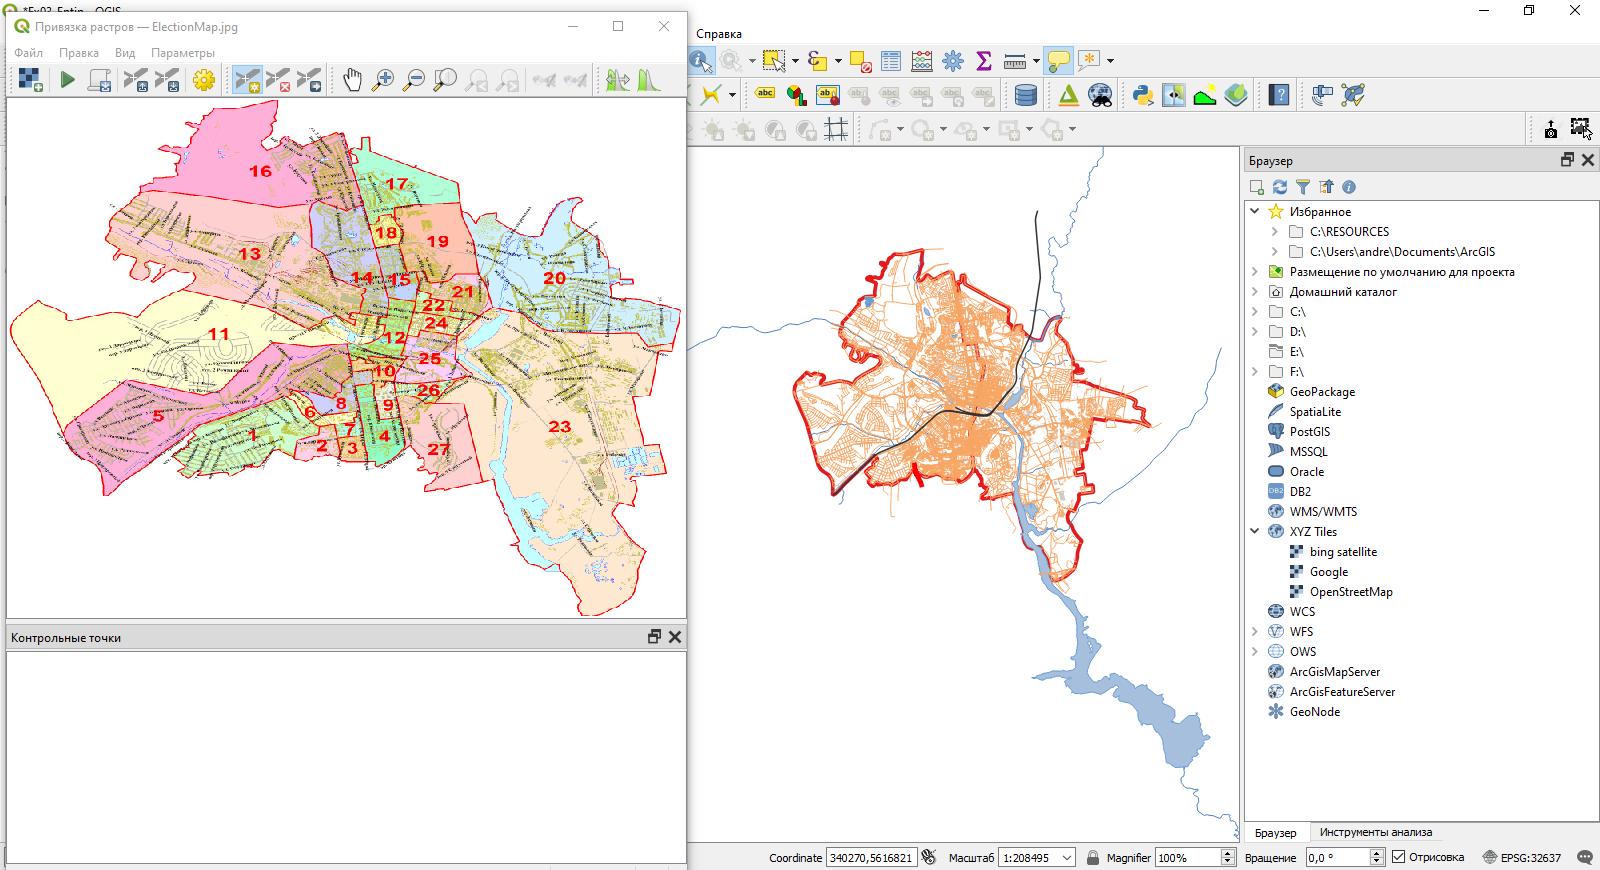
\includegraphics{images/Ex05/Reference1.png}

  Обратите внимание, что растровое изображение выглядит искажённым («сплюснутым») по сравнению с изображением в основном окне QGIS. Если вы откроете растр в какой-либо программе просмотра изображений, вы убедитесь, что растр действительно будто бы «сжат» по вертикали.
\item
  Перемещаясь по карте, найдите соответствующие точки на изображении и в основном окне QGIS

  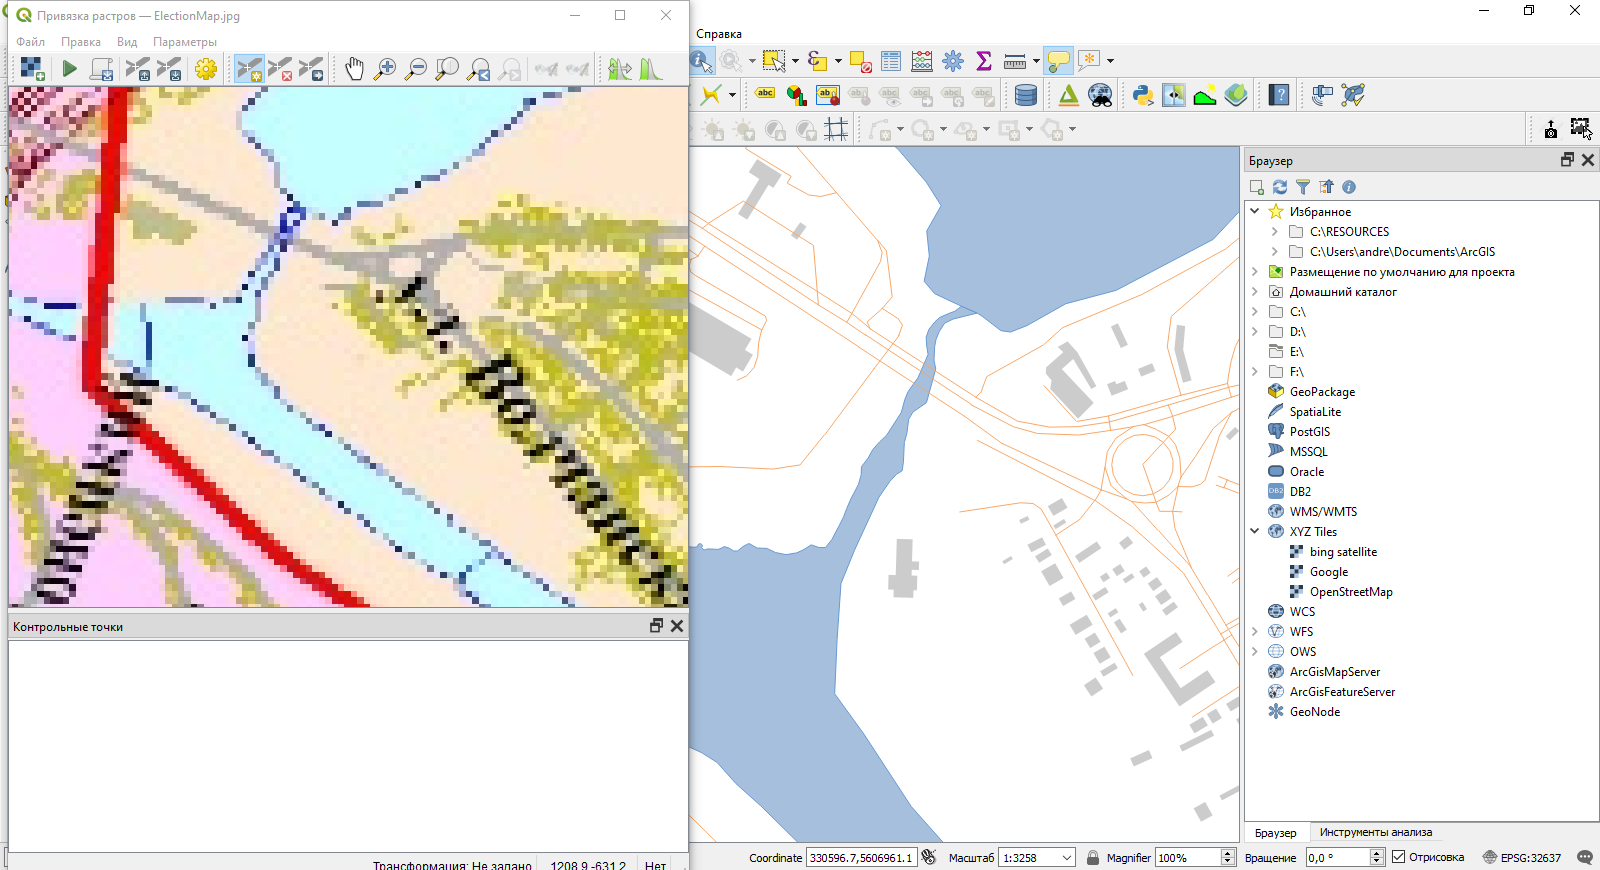
\includegraphics{images/Ex05/Reference2.png}
\item
  Используя инструмент «Добавить точку» в окне модуля привязки, установите первую точку на растровом изображении (щелчком левой кнопки мыши). QGIS выдаст запрос на ввод координат:

  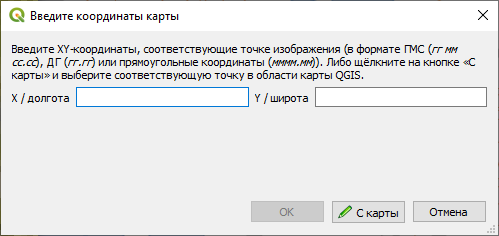
\includegraphics{images/Ex05/Reference3.png}
\item
  В некоторых случаях можно ввести координаты вручную, но нам будет проще «снять их с карты», то есть указать соответственную точку в основном окне QGIS. Нажмите кнопку «С карты». Окна модуля привязки при этом свернутся.
\item
  Щёлкните левой кнопкой мыше в соответствующей точке основного окна QGIS. Программа автоматически считает координаты точки и подставит их в форму:

  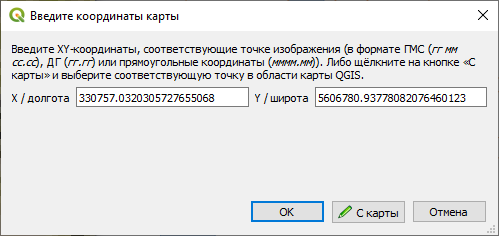
\includegraphics{images/Ex05/Reference4.png}
\item
  Нажмите OK, чтобы добавить первую опорную точку.

  \begin{quote}
  Примечание: счёт опорных точек в QGIS начинается с нуля, поэтому первая точка получит индекс «0», вторая --- «1» и так далее.
  \end{quote}
\item
  \textbf{Найдите и расставьте ещё 7-8 опорных точек.}. Точки должны быть равномерно распределены по полю карты и не находиться на одной линии. В качестве опорных точек лучше всего использовать пересечения автодорог и/или железных дорог. Кроме того, не следует использовать контура границ для расстановки опорных точек --- в представленных материалах они не совпадают!
\item
  Откройте окно параметров трансформации 
\includegraphics{images/Ex05/parameters.png} и ознакомьтесь с доступными параметрами трансформации.

  \textbf{Вопрос 2:} какие типы трансформации растра доступны в QGIS? В каких случаях они применяются? Сколько точек необходимо для осуществления каждого типа трансформации?
\item
  Настройте параметры трансформации следующим образом:

  \begin{itemize}
  \tightlist
  \item
    \textbf{Тип трансформации:} Проективная;
  \item
    \textbf{Метод интерполяции:} Ближайший сосед;
  \item
    \textbf{Целевая система координат:} такая же, как СК проекта;
  \item
    Остальные параметры оставьте по умолчанию
  \item
    Обязательно включите опцию «Открыть результат в QGIS»
  \end{itemize}
\item
  Нажмите ОК, чтобы закрыть окно параметров трансформации и сохранить изменения настроек.
\item
  Изучите таблицу опорных точек, которая отображается внизу окна модуля привязки. Если суммарная невязка для какой-либо точки превышает 0,5 пикселя, отключите её и добавьте новую точку. Не удаляйте отключённые точки!

  \begin{quote}
  Подсказка: чтобы легче было ориентироваться в опорных точках, можно включить отображение идентификаторов точек в настройках модуля привязки.
  \end{quote}

  \textbf{Вопрос 3:} Можно ли загружать и сохранять опорные точки привязки в QGIS? Если да, как это сделать?
\item
  Когда точность всех активных опорных точек составит меньше 1 пикселя, нажмите кнопку 
\includegraphics{images/Ex05/go.png}, чтобы запустить процесс привязки. В результате будет создан новый файл, который автоматически добавится в основное окно QGIS.
\item
  Изучите результат привязки. Если он устраивает вас, окно привязки можно закрывать. Если нет, удалите добавленный слой, вернитесь в окно привязки, внесите необходимые изменения и запустите привязку ещё раз.

  \textbf{Скриншот 2:} окно QGIS после завершения привязки.
\end{enumerate}

\hypertarget{map-ref-districts-creation}{%
\section{Создание слоя избирательных округов}\label{map-ref-districts-creation}}

\protect\hyperlink{map-ref-districts}{В начало упражнения ⇡}

\begin{enumerate}
\def\labelenumi{\arabic{enumi}.}
\item
  Отключите все слои, кроме административных границ. Измените стиль слоя границ на \texttt{outline\ black}. Разместите привязанный растр в таблице слоёв под слоем административных границ.

  Мы готовы к тому, чтобы начать векторизовать («цифровать») контура избирательных округов. Но для этого нам нужен набор данных, в который мы будем сохранять создаваемые объекты. На следующем шаге мы создадим такой набор данных.
\item
  \textbf{Создайте новый набор данных GeoPackage}. Это можно сделать из панели источников данных, из меню «слой» или нажав комбинацию клавиш \texttt{Ctrl+Shift+N}. Откроется окно настройки нового слоя.
\item
  Заполните поля в открывшемся окне следующим образом:

  \begin{itemize}
  \tightlist
  \item
    \textbf{База данных:} сохраните файл \texttt{*.gpkg} в папку \texttt{Ex05\_RefAdm}. Назовите его по шаблону \texttt{Belgorod\_\%фамилия\%.gpkg};
  \item
    \textbf{Имя таблицы:} примите значение, предлагаемое по умолчанию после указания пути к базе;
  \item
    \textbf{Тип геометрии:} \emph{(определите самостоятельно)}
  \item
    Чекбоксы «Include Z dimension» и «Include M values» оставьте выключенными;
  \item
    \textbf{Система координат}: такая же, как система координат проекта.
  \end{itemize}
\item
  Блоки \emph{New Field} и \emph{Fields List} предназначены для настройки таблицы атрибутов создаваемого набора данных. В блоке \emph{New Field} вводится имя, тип и длина поля, по нажатию кнопки \emph{Add to Fields list} создаваемое поле добавляется в список.

  Добавьте поле \textbf{district\_id} целочисленного типа в список полей.

  не раскрывайте блок \emph{Advanced Options}, они не интересуют нас в рамках этого упражнения.

  После применения всех настроек окно создания нового набора будет выглядеть аналогично представленному на экране:

  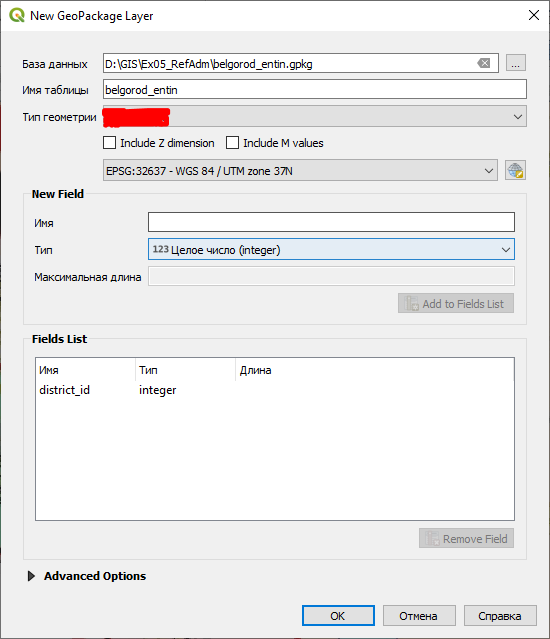
\includegraphics{images/Ex05/NewGeoPackage.png}
\item
  Нажмите ОК, чтобы создать источник данных. Новый слой автоматически добавится в проект.

  На следующих шагах вы будете создавать новые пространственные объекты в этом слое.
\item
  Измените стиль слоя на \texttt{pattern\ dot\ red}. Такая символика удобна для цифрования, поскольку позволит не «скрывать» растровый слой под созданными объектами.
\item
  Редактирование данных в ГИС по умолчанию «выключено». Чтобы получить возможность редактировать наборы данных, нужно включать специальный режим редактирования. В QGIS этот режим включается отдельно для каждого слоя. Чтобы включить режим редактирования, выберите слой, который вы собираетесь редактировать, в таблице слоёв и нажмите кнопку 
\includegraphics{images/Ex05/Editing1.png} на панели инструментов оцифровки.
\item
  Включив режим редактирования, нажмите кнопку «Добавить объект» 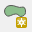
\includegraphics{images/Ex05/Editing2.png} в панели инструментов оцифровки, чтобы добавить новый объект. Внешний вид и название этой кнопки будут отличаться в зависимости от типа геометрии слоя.
\item
  Включите панель инструментов прилипания, если она ещё не включена.

  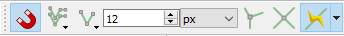
\includegraphics{images/Ex05/snapping.png}

  \begin{quote}
  Примечание: прилипание (\emph{snapping}, снеппинг) и его частный случай --- трассировка (\emph{tracing}) --- исключительно важные функции программных средств ГИС. Они позволяют повторять контура уже существующих объектов при редактировании. Это не только ускоряет процесс, но и позволяет соблюдать специфические геоинформационные требования к топологии пространственных данных.
  \end{quote}
\item
  В панели инструментов прилипания:

  \begin{itemize}
  \tightlist
  \item
    Включите прилипание;
  \item
    Установите режим прилипания «к вершинам и сегментам»
  \item
    Порог прилипания --- не меньше 10 пикселей
  \item
    Включите трассировку (\emph{Tracing})
  \end{itemize}

  Эти настройки нужны, чтобы контура создаваемых вами объектов повторяли контура слоя административных границ, где это необходимо.

  Теперь вы готовы к тому, чтобы оцифровать свой первый контур. Ваша задача будет состоять в том, чтобы оцифровать границы избирательных округов в пределах одного из административных округов Белгорода (Западного или Восточного).
\item
  Увеличьте изображение таким образом, чтобы видеть избирательные округа возле южного сегмента границы двух административных округов. Нажмите левой кнопкой мыши на карте в месте, где проходит граница избирательного округа и не проходит граница административного округа. По нажатию левой кнопки мыши устанавливается положение первого узла создаваемого контура.
\item
  «Обходите» контур по часовой стрелке или против часовой стрелки, устанавливая новые узлы.

  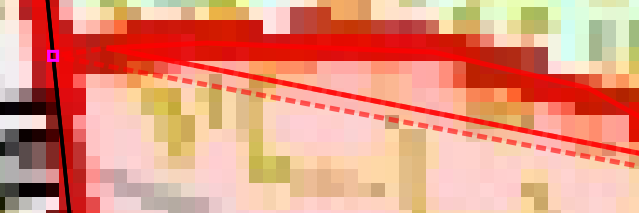
\includegraphics{images/Ex05/Editing4.png}

  Не пугайтесь, если QGIS отобразит зелёный крестик поверх вашего контура --- таким образом маркируются самопересечения.

  Чтобы удалить последний введённый узел, нажмите \texttt{Backspace}. Чтобы сбросить контур целиком, нажмите \texttt{Esc}.
\item
  Дойдя до границы административных округов, установите новый узел на ней. Место установки узла автоматически притянется к границе.

  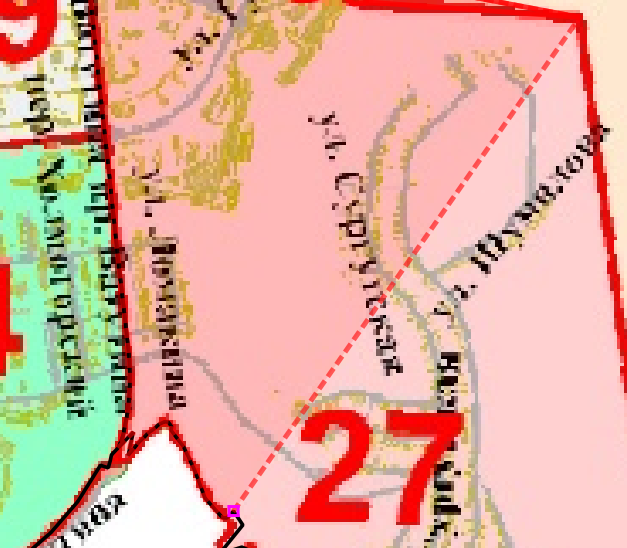
\includegraphics{images/Ex05/Editing5.png}
\item
  Теперь переместите курсор вдоль границы. Наблюдайте за тем, как ориентируется контур создаваемого объекта. Установите следующий узел на границе подальше от точки касания.

  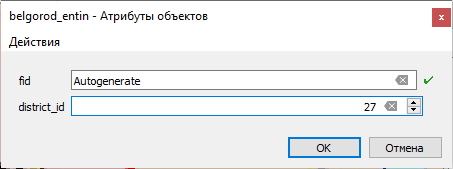
\includegraphics{images/Ex05/Editing6.png}
\item
  Когда границы округов «разойдутся», снова нажимайте левую кнопку мыши, чтобы установить новый узел в желаемой точке.
\item
  Чтобы завершить редактирование, нажмите правую кнопку мыши. Откроется окно ввода атрибутов. Введите номер избирательного округа и нажмите ОК или Enter, чтобы применить изменения и закрыть окно ввода атрибутов.

  Новый объект добавлен в слой и отображается на карте.

  \begin{quote}
  Примечание: неправильно введённый номер можно исправить в таблице атрибутов
  \end{quote}
\item
  Векторизуйте остальные объекты в пределах выделенной вам половины г. Белгорода. Следуйте границам административных округов и ранее оцифрованных объектах. При незначительных различиях в границах цифруйте по границам административных округов, если расхождения большие --- цифруйте по границам избирательных округов.
\item
  Сохраните изменения в слое. Для этого нажмите кнопку «Сохранить правки» 
\includegraphics{images/Ex05/Editing7.png} на панели инструментов оцифровки. Не выключайте режим редактирования.

  \begin{quote}
  Примечание: сохранение правок в слое никак не сказывается на сохранении проекта и независимо от него. Вы можете сохранить проект, затем в другом проекте изменить один из наборов пространственных данных, затем вернуться в изначальный проект --- и все изменения набора отобразятся в нём. На символику слоя это не повлияет.
  \end{quote}
\item
  Отключите растровый слой. Включите для набора данных об избирательных округах подписи по полю \texttt{district\_id}. Настройки подписей задайте самостоятельно.

  \textbf{Скриншот 3:} оцифрованные контура избирательных округов.
\end{enumerate}

\hypertarget{map-ref-districts-stats}{%
\section{Расчет статистики по округам}\label{map-ref-districts-stats}}

\protect\hyperlink{map-ref-districts}{В начало упражнения ⇡}

В данной части работы предлагается определить количество зданий разных типов (жилые многоэтажки и частная застройка), которые попадают в пределы каждого округа, затем построить картодиаграммы по полученным значениям. Для этого будет использован следующий алгоритм:

\begin{itemize}
\item
  Выбрать округ на карте
\item
  Выбрать здания, попадающие в его пределы (\emph{пространственный запрос}).
\item
  Из полученной выборки оставить только здания, принадлежащие к определённому типу (\emph{атрибутивный запрос}).
\item
  Записать число отобранных зданий в соответствующий атрибут текущего района.
\end{itemize}

Эти операции необходимо повторить для каждого округа.

\begin{enumerate}
\def\labelenumi{\arabic{enumi}.}
\item
  Не выключая режим редактирования, откройте таблицу атрибутов слоя.
\item
  Нажмите кнопку «Добавить новое поле» или \texttt{Ctrl+W} на клавиатуре, чтобы добавить новый столбец в таблицу.
\item
  Добавьте два целочисленных поля: \texttt{count\_apartments} и \texttt{count\_house}. Эти поля будут служить для подсчёта (\emph{count}) многоквартирных жилых домов (\emph{apartments}) и частной застройки (\emph{house}) соответственно.
\item
  Включите слой зданий.
\item
  \textbf{Выберите} первый созданный вами контур округа: выделите строку в таблице атрибутов или воспользуйтесь инструментом выборки в окне карты 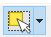
\includegraphics{images/Ex05/selection1.png}. Выделенный объект будет подсвечен жёлтым цветом на карте и синим --- в таблице атрибутов.
\item
  Теперь выберите те объекты из слоя зданий, которые находятся внутри выбранного округа. Для этого запустите инструмент «Вектор» --- «Выборка» --- «Выделение по районам\ldots». Используйте условие «находятся внутри» (\emph{are within}).

  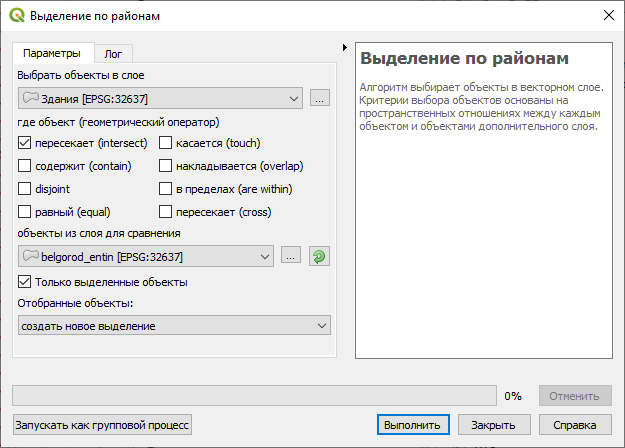
\includegraphics{images/Ex05/selection2.png}

  Нажмите «Выполнить», чтобы выбрать объекты в слое зданий.
\item
  Имея выборку в слое зданий и не закрывая окно пространственного запроса («Выделение по районам\ldots»), осуществите выборку по атрибутам. Для этого выберите в таблице слоёв слой зданий и нажмите кнопку «Выделить объекты, удовлетворяющие условию» 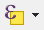
\includegraphics{images/Ex05/selection3.png}. Откроется форма ввода атрибутивного запроса.

  \begin{quote}
  Атрибутивные запросы в ГИС, как правило, создаются с использованием диалектов языка \href{https://ru.wikipedia.org/wiki/SQL}{SQL}. Само выражение представляет собой только условие (\emph{where clause}) и часто использует значения атрибутов.
  \end{quote}
\item
  Форма ввода атрибутивного запроса состоит из трёх частей. В левой части конструируется собственно запрос, средняя содержит список доступных переменных и функций, в правой отображается справочная и служебная информация.
\item
  В структуре тегов OpenStreetMap многоэтажные жилые дома обозначаются тегом \texttt{apartments}. После конвертации данных OpenStreetMap в реляционную базу данных соответствующий тег содержится в поле \texttt{buildings}.

  Мы должны \textbf{выбрать} в слое зданий те объекты, значение атрибута \texttt{buildings} которых задано как \texttt{apartments}.
\item
  Найдите в среднем поле группу «Поля и значения» и разверните её. Найдите поле «Building» и дважды щёлкните по нему левой кнопкой мыши. Поле будет добавлено в запрос, в нижней части окна появится пример результата запроса, а в правой части отобразится вспомогательная форма извлечения уникальных значений.
\item
  Введите знак \texttt{=} в поле конструирования запроса.
\item
  Нажмите кнопку \emph{All Unique}, чтобы получить список уникальных значений, записанных в поле \texttt{building}.
\item
  Дважды щёлкните по записи \texttt{apartments} в списке уникальных значений. Она будет добавлена в конструктор запроса.

  После применения всех действий окно конструктора запроса будет выглядеть, как на рисунке ниже:

  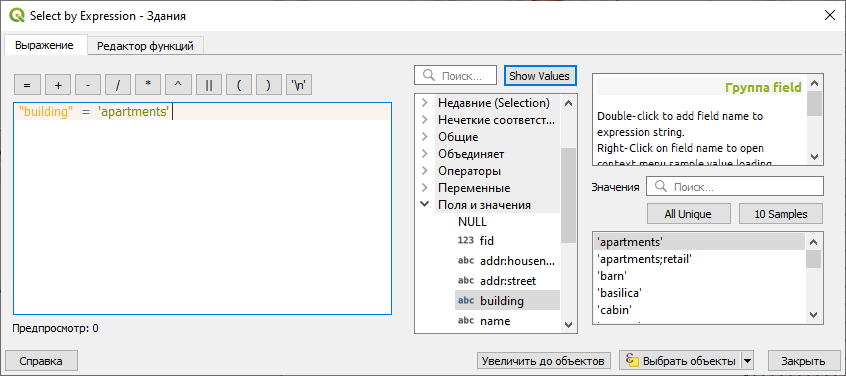
\includegraphics{images/Ex05/selection4.png}

  \textbf{Вопрос 4:} Почему в нижней части окна отображается запись «Предпросмотр: 0»?
\item
  Мы сформулировали условие для выборки, однако нам нужно выбрать объекты не просто из слоя, а из уже существующей выборки. Для этого откройте выпадающий список кнопки «Выбрать объекты» и выберите функцию «Фильтровать текущее выделение»:

  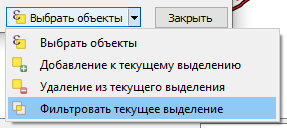
\includegraphics{images/Ex05/selection5.png}
\item
  После применения фильтра появится всплывающее сообщение с числом выбранных объектов. Эта информация будет продублирована внизу окна QGIS:

  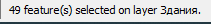
\includegraphics{images/Ex05/selection6.png}
\item
  Введите полученную цифру в таблицу атрибутов слоя избирательных округов.
\item
  Повторите выборку поочерёдно для каждого округа. Вводите получаемые значения в таблицу атрибутов. Не забывайте периодически сохранять изменения!
\item
  Теперь повторите выборку ещё раз, но уже не для многоквартирных домов, а для частных владений. Им соответствует запись \texttt{house} в поле \texttt{building}.

  \textbf{Вопрос 5:} вставьте в отчёт SQL-выражение для выбора частных владений.

  \textbf{Вопрос 6:} можно ли было делать выборку в другом порядке (т.е. сначала выборку по атрибутам, а затем --- по пространственному положению)? Если да, то каковы были бы отличия процедуры?
\item
  Скопируйте таблицу атрибутов в любой табличный процессор (Microsoft Excel, Google Sheets, LibreOffice Calc). Для этого при помощи сочетания клавиш \texttt{Ctrl+A} выделите все записи в таблице, скопируйте при помощи \texttt{Ctrl+C} и вставьте записи без форматирования в табличный процессор при помощи \texttt{Ctrl+Shift+V}.
\item
  Удалите первый столбец (\texttt{wkt\_geometry}).
\item
  \textbf{Скопируйте остальные столбцы и вставьте их в отчётный файл}.
\end{enumerate}

\hypertarget{map-ref-districts-diagrams}{%
\section{Построение картодиаграмм}\label{map-ref-districts-diagrams}}

\protect\hyperlink{map-ref-districts}{В начало упражнения ⇡}

Диаграммы в QGIS создаются как настройка отображения слоя. Однако соответствующий блок располагается не на вкладке «Стиль», как «обычные» условные знаки, а на отдельной вкладке «Диаграммы».

Инструменты создания диаграмм в QGIS пока ещё несовершенны и находятся в стадии активной разработки, поэтому, во-первых, некоторые настройки могут работать некорректно, во-вторых, в скором будущем возможно кардинальное изменение интерфейса настройки.

\begin{enumerate}
\def\labelenumi{\arabic{enumi}.}
\item
  Откройте свойства слоя избирательных округов и перейдите на вкладку «Диаграммы». В верхнем левом углу включите отображение круговых диаграмм.
\item
  На вкладке «Атрибуты» добавьте атрибуты \texttt{count\_apartments} и \texttt{count\_house} в список включённых в диаграмму. Настройте мягкие, пастельные цвета для их отображения.
\item
  Вкладку «Рендеринг» установите для диаграмм настройку прозрачности (70 \%)
\item
  На вкладке «Размер» измените способ задания размера с фиксированного на переменный («масштабируемый»).

  Изменение размера диаграмм в QGIS работает следующим образом. Пользователь задаёт максимальное значение показателя, который будет управлять размером диаграммы, и соответствующий ему максимальный диаметр диаграммы. Размер круга масштабируется пропорционально величине показателя. Из картографических соображений следует всегда выбирать масштабирование площади, а не линейного размера (диаметра).

  В качестве показателя можно использовать значение из какого-либо столбца таблицы атрибутов. Но можно и рассчитывать это значение непосредственно при визуализации. Мы воспользуемся вторым вариантом.
\item
  Нажмите кнопку со значком в виде буквы ε справа от поля «Атрибут». Откроется уже знакомое вам окно конструирования выражений.
\item
  Задайте выражение для суммирования значений полей \texttt{count\_apartments} и \texttt{count\_house}. Убедитесь, что расчёт выполняется кооректно (см. строку «Предпросмотр») и, если это так, нажмите OK.
\item
  Вернувшись в окно настройки диаграмм, нажмите кнопку «Найти» в строке «Максимальное значение», чтобы автоматически рассчитать максимальный результат выражения.
\item
  Округлите полученное значение в большую сторону до тысяч.
\item
  Установите максимальный размер диаграмм равным 30 (мм).

  В QGIS есть ещё одна полезная опция --- увеличение размера диаграмм. Она применяется, если при масштабировании некоторые диаграммы становятся слишком малы. В таком случае их размер увеличивается до минимального (задаваемого пользователем) порогового значения.

  После установки всех параметров окно должно принять следующий вид:

  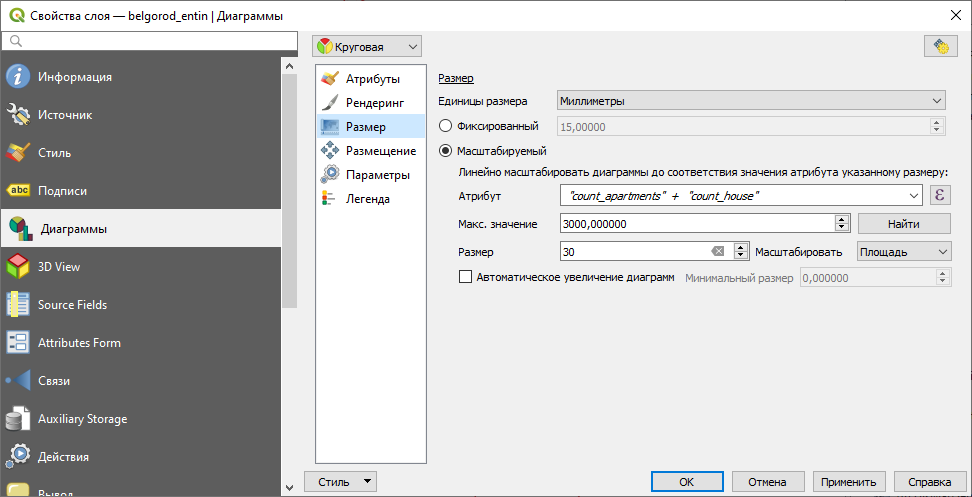
\includegraphics{images/Ex05/diagram1.png}
\item
  Перейдите на вкладку «Легенда». Здесь вы настроите комбинацию условных знаков для отображения в легенде. Нажмите кнопку «Показать значки для размера диаграмм в легенде» (\emph{Show Legend Entries for Diagram Size}).
\item
  Настройте отображение значков следующим образом:

  \begin{itemize}
  \tightlist
  \item
    «Коллапсируйте» значки легенды;
  \item
    В качестве символа используйте белый маркер круглой формы с тёмно-серой обводкой;
  \item
    Задайте заголовок («Число домов»);
  \item
    Задайте классы значков вручную: 100, 500, 1000, далее через 1000 до максимальной величины.
  \end{itemize}

  Интерфейс настройки диаграммы должен принять приблизительно следующий вид:

  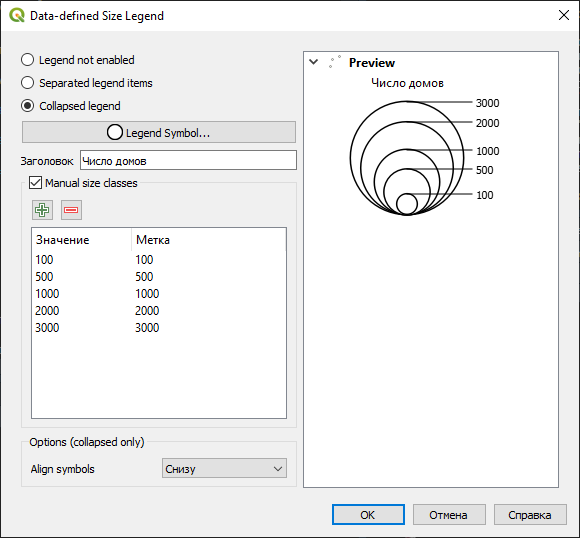
\includegraphics{images/Ex05/diagram2.png}

  \begin{quote}
  \textbf{Важное замечание:} конечно, такой набор значков не является картографически корректным для создания легенды к абсолютной непрерывной шкале значков. По состоянию на 2020-03-18 ни один широко используемый ГИС-пакет не может сделать легенду к размерам кругов картодиаграммы согласно принятым картографическим правилам. Легенды к таким картам следует составлять или исправлять вручную.
  \end{quote}
\end{enumerate}

\hypertarget{map-ref-districts-wms}{%
\section{Использование базовых слоёв из сети Интернет}\label{map-ref-districts-wms}}

\protect\hyperlink{map-ref-districts}{В начало упражнения ⇡}

Большинство современных программных средств ГИС даёт возможность использовать не только локальные данные, но и наборы, распространяемые через Интернет с использованием специальных протоколов (WMS, WFS, WCS и др.). В частности, таким способом можно добавлять в ваш проект базовые карты Google Maps, Яндекс.Карт и некоторых других сервисов.

Разработан удобный плагин, позволяющий вам получить доступ к этим источникам «в один клик». Он называется \textbf{QuickMapServices}.

\begin{enumerate}
\def\labelenumi{\arabic{enumi}.}
\item
  Откройте меню управления подключаемыми модулями («Модули» --- «Управление модулями\ldots»), наберите в строке поиска \texttt{QuickMapServices} и установите найденный модуль.

  Установленный модуль будет доступен из выпадающего меню «Интернет»:

  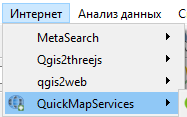
\includegraphics{images/Ex05/qms1.png}
\item
  Откройте настройки модуля \emph{QuickMapServices}, перейдите на вкладку «Загрузить сервисы» и нажмите «Получить дополнительные источники данных». В список доступных сервисов добавится ряд дополнительных источников.

  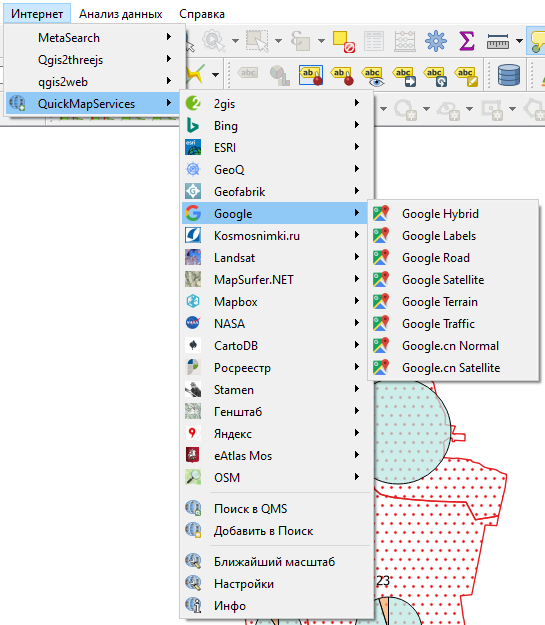
\includegraphics{images/Ex05/qms2.png}
\item
  Добавьте к проекту базовую карту OpenStreetMap Monochrome.
\item
  Расположите слой с избирательными округами поверх базовой карты. Все остальные слои отключите.
\end{enumerate}

\hypertarget{map-ref-districts-result}{%
\section{Оформление итоговой схемы}\label{map-ref-districts-result}}

\protect\hyperlink{map-ref-districts}{В начало упражнения ⇡}

\begin{enumerate}
\def\labelenumi{\arabic{enumi}.}
\item
  Создайте макет компоновки для оформления итоговой схемы.
\item
  Добавьте карту к макету. Настройте оформление карты. Исходите из того, что ваша схема предназначена для вставки в отчёт: учтите ориентировку страницы, необходимость зарезервировать место под поля и др.

  В рамках этого упражнения не создавайте сетку координат, но добавьте рамку карты и отключите фон.
\item
  Добавьте легенду и настройте её.
\item
  Добавьте остальные необходимые элементы зарамочного оформления.
\item
  Оцените получившееся изображение. При необходимости вернитесь в основное окно QGIS и измените настройки оформления слоёв.
\item
  Экспортируйте схему с разрешением 96 точек на дюйм. Используйте опцию «Обрезать по содержимому».

  \begin{quote}
  Примечание: разрешение 96 точек на дюйм считается довольно низким для картографических целей. Изображения с таким разрешением не годятся для печати, но иногда могут быть пригодны для размещения в Интернете. ВЫ снижаете разрешение для того, чтобы сохранить читаемость базовой карты.
  \end{quote}
\item
  Вставьте итоговую схему в отчётный файл.
\end{enumerate}

\hypertarget{overlay}{%
\chapter{Анализ пространственных взаимосвязей}\label{overlay}}

\href{http://autolab.geogr.msu.ru/gis/data/Ex10.zip}{Скачать данные и файл отчета}

\hypertarget{overlay-intro}{%
\section{Введение}\label{overlay-intro}}

\textbf{Цель задания} --- научиться определять пространственную приуроченность двух явлений на основе процента взаимного покрытия их площадей (методом оверлея).

\textbf{Необходимая теоретическая подготовка:} Оверлей пространственных объектов, геометрическое определение вероятности как отношения мер (площадей), соединение таблиц в реляционных базах данных, внешний и внутренний ключ соединения.

\textbf{Необходимая практическая подготовка:} Знание основных компонент интерфейса QGIS (менеджер источников данных, таблица слоёв, фрейм карты, менеджер компоновок). Работа с различными форматами источников пространственных данных . Настройка символики и подписей объектов. Владение базовыми ГИС-технологиями.

\textbf{Исходные данные:} База данных ГИС «Сатино».

\textbf{Результат:} Таблица взаимного покрытия площадей типов рельефа и подтипов почв.

\hypertarget{overlay-control}{%
\subsection{Контрольный лист}\label{overlay-control}}

\begin{itemize}
\tightlist
\item
  Добавить на карту слои типов почв и рельефа, оформить их
\item
  Произвести оверлей слоев
\item
  Произвести слияние данных и соединение таблиц
\item
  Подсчитать процент покрытия площадей
\end{itemize}

\hypertarget{overlay-annotation}{%
\subsection{Аннотация}\label{overlay-annotation}}

Задание посвящено знакомству с пространственным анализом на основе векторных данных. Векторная модель представляет объекты в виде отдельных геометрических фигур с набором атрибутов. Она является объектно-ориентированной и удобна для анализа формы, размеров объектов, их взаимной конфигурации в пространстве. Одним из широко используемых методов анализа на основе векторных данных является оверлей.

\begin{quote}
При \emph{оверлее} происходит наложение двух или более слоев, в результате чего образуется их графическая композиция. Полученные участки наследуют атрибуты от каждого слоя. Эта операция базируется на стандартных отношениях множеств, таких как пересечение, объединение и симметрическая разность.
\end{quote}

С помощью оверлея можно, например, установить, к каким генетическим типам рельефа приурочены различные типы и подтипы почв. В общем случае оверлей позволяет установить, какие комбинации объектов встречаются в пространстве. В задании предлагается исследовать методом оверлея взаимосвязь типов рельефа и типов и подтипов почв.

\hypertarget{overlay-vectors}{%
\section{Визуальный анализ векторных слоев}\label{overlay-vectors}}

\protect\hyperlink{overlay}{В начало упражнения ⇡}

В первую очередь при анализе данных следует провести их визуальную оценку, которая может натолкнуть на отыскание закономерностей во взаимном расположении объектов.

\begin{enumerate}
\def\labelenumi{\arabic{enumi}.}
\item
  Распакуйте архив с материалами упражнения в свою рабочую директорию. Создайте проект QGIS в папке с распакованными материалами.
\item
  Добавьте на карту слой \emph{RelTypes} из базы геоданных \texttt{Satino.gdb}. Примените к нему стиль из файла \texttt{RelTypes.qml}.

  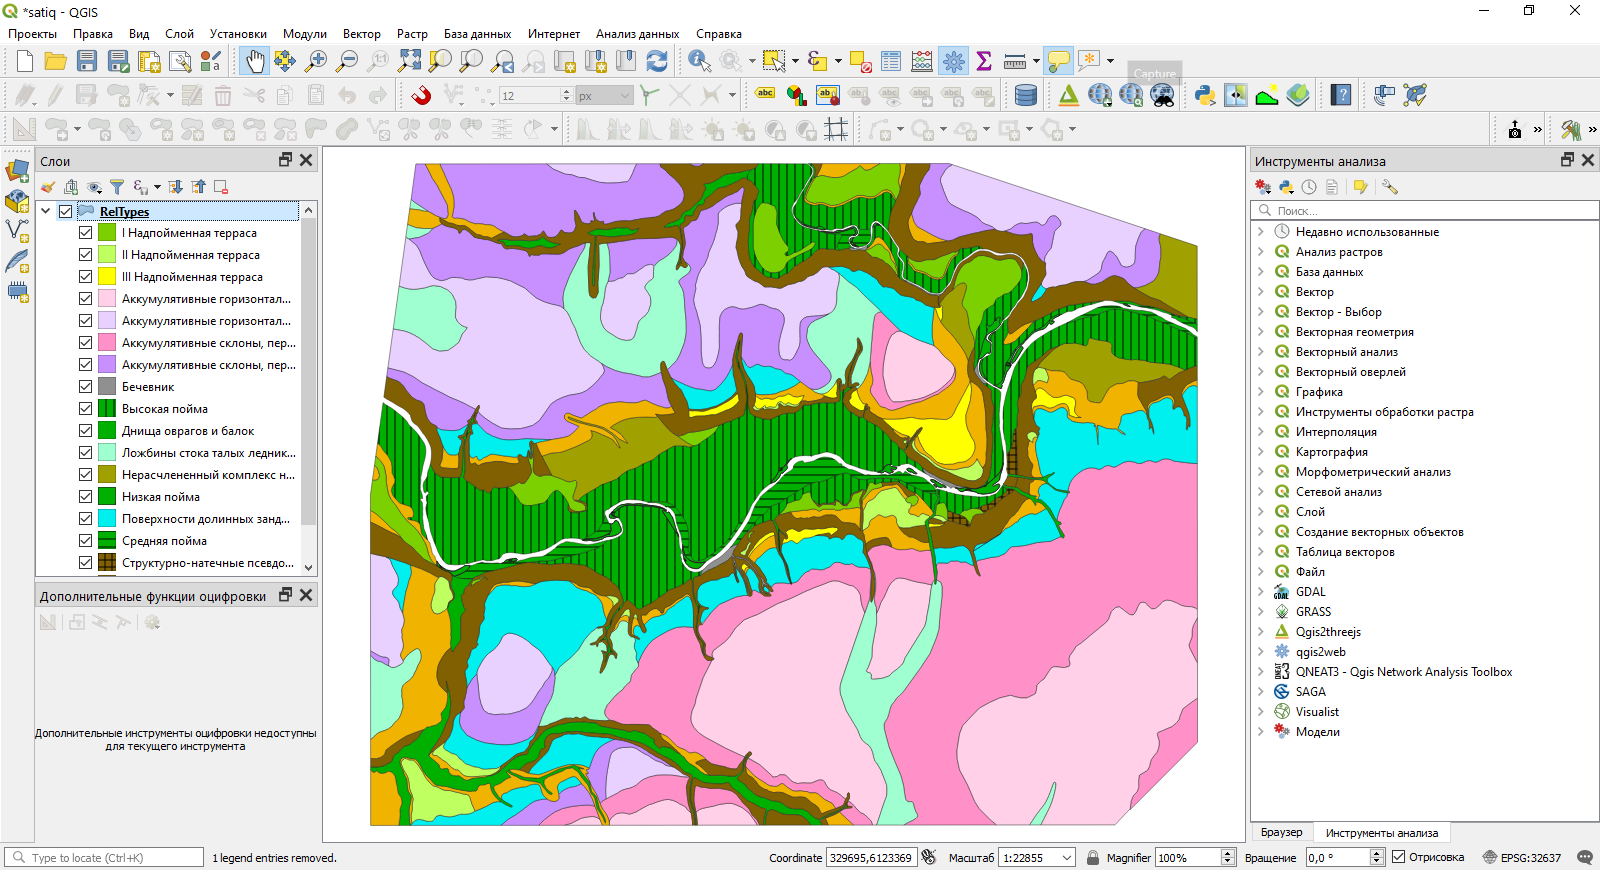
\includegraphics{images/Ex06/AppliedStyle1.png}
\item
  Добавьте на карту слой \emph{SoilTypes} из той же базы. Изобразите его в виде полигонов без заливки с обводкой красного цвета.

  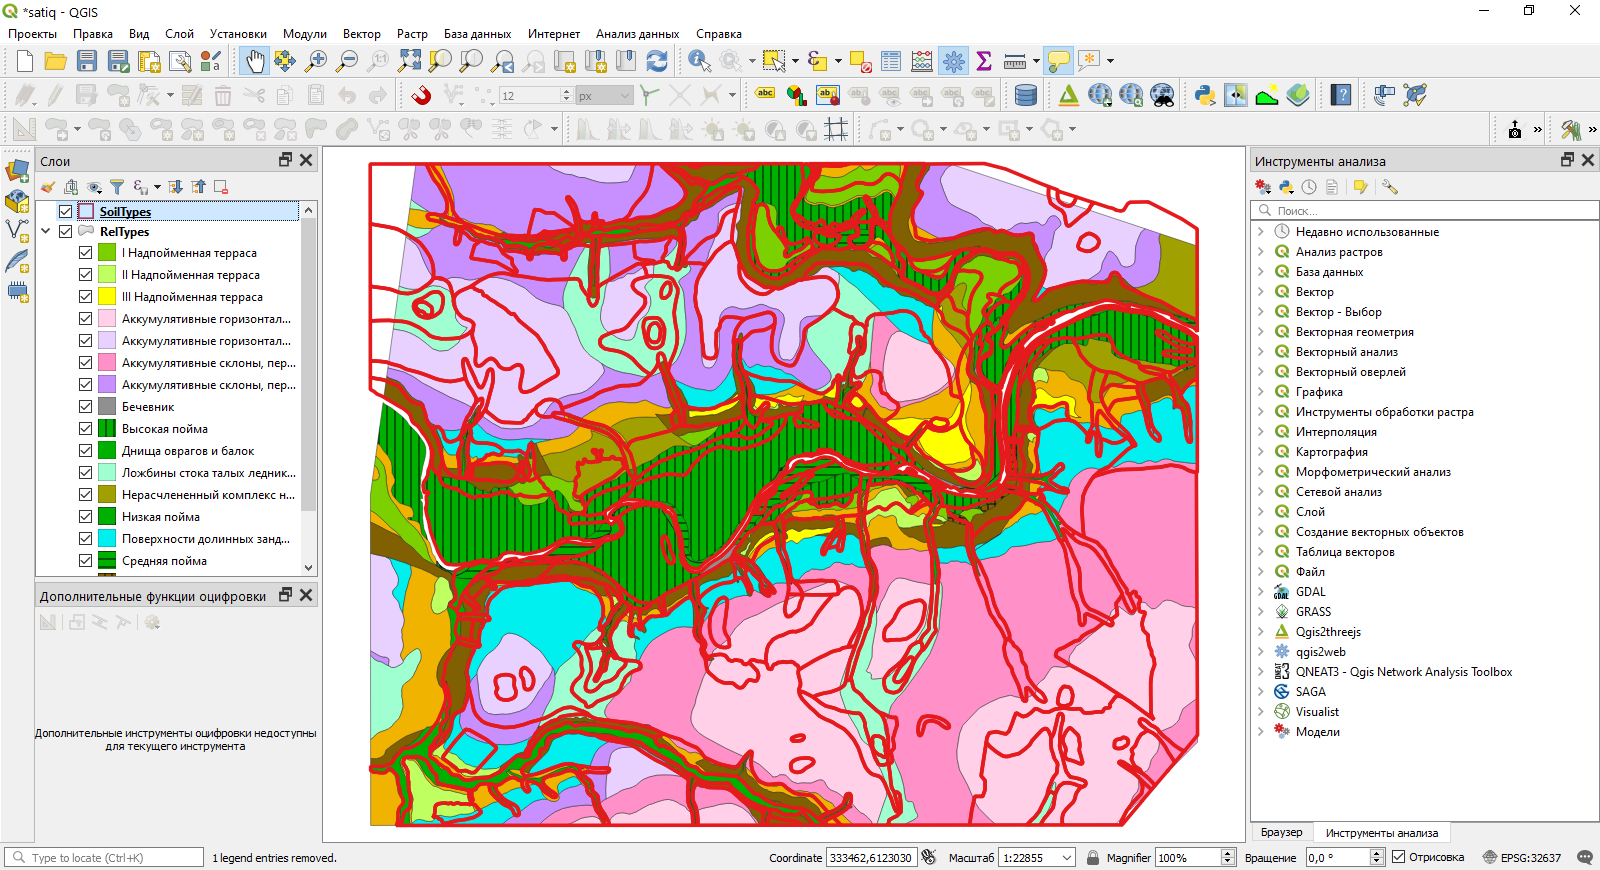
\includegraphics{images/Ex06/AppliedStyle2.png}
\item
  Выберите инструмент идентификации 
\includegraphics{images/Ex06/icon_identify.png} и щелкните в пределах карты на любом полигоне. Откроется форма идентификации (отображения) атрибутов объекта

  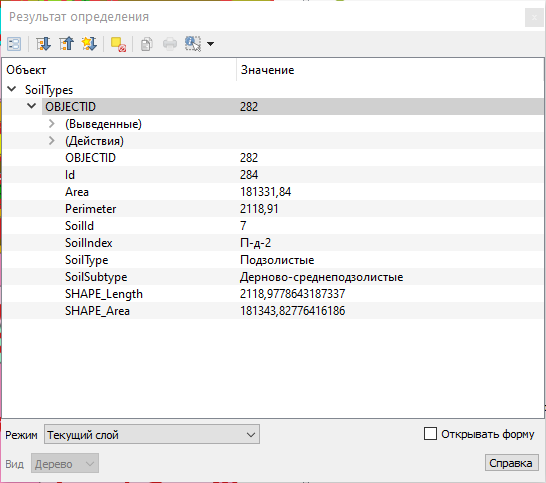
\includegraphics{images/Ex06/identify1.png}

  По умолчанию QGIS идентифицирует объекты либо из самого верхнего слоя (\emph{Сверху вниз, до первого найденного}, в порядке перечисления в панели слоёв), либо из того слоя, который выбран в панели слоёв (\emph{Текущий слой}). Можно настроить инструмент идентификации таким образом, чтобы отображать атрибуты объектов из всех доступных слоёв. Для этого в нижней части панели идентификации нужно установить режим \emph{Сверху вниз}.

  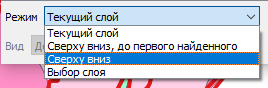
\includegraphics{images/Ex06/identify2.png}

  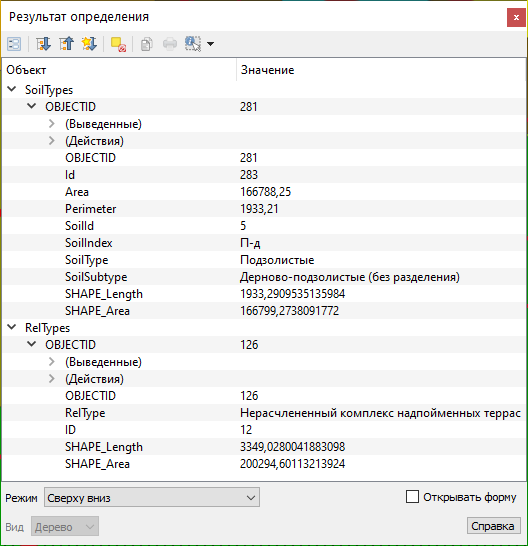
\includegraphics{images/Ex06/identify3.png}

  Пользуясь инструментом идентификации, проанализируйте совмещенное изображение границ типов почв и рельефа.
\end{enumerate}

\textbf{Вопрос 1:} Есть ли какие-то совпадения или подобия рисунков контуров типов рельефа и подтипов почв в пределах речных долин, междуречий, малых эрозионных форм?

Когда данные исследованы визуально и путем идентификации, можно перейти к их анализу с помощью оверлея.

\hypertarget{overlay-intersect}{%
\section{Оверлей слоев методом пересечения}\label{overlay-intersect}}

\protect\hyperlink{overlay}{В начало упражнения ⇡}

Инструменты векторного оверлея, а также некоторые родственные им инструменты в QGIS размещаются в меню «Вектор --- Геообработка». Также эти инструменты доступны из панели инструментов анализа.

\emph{Изучите, как работают инструменты геообработки}. Для этого сохраните и закройте свой проект QGIS, затем создайте новый проект, а в нём --- два временных полигональных слоя.

\begin{quote}
Временный слой в QGIS хранится в выделенной директории среди системных файлов. Если не сохранять временные файлы, они будут удалены после закрытия окна QGIS.
\end{quote}

\begin{quote}
Чтобы создать временный слой, нажмите кнопку \emph{Новый временный слой} в панели менеджера источников данных. Используйте для создаваемых слоёв проецированную систему координат!
\end{quote}

\textbf{поочерёдно примените к вашим слоям следующие инструменты геообработки: Обрезать (Clip), Разность (Erase), пересечение (Intersect), Симметрическая разность (Symmetrical Difference), Объединение (Union)} и ответьте на вопросы:

\textbf{Вопрос 2}: опишите словесно, как будет выглядеть результат применения каждого из инструментов геообработки к произвольной паре наборов данных?

\textbf{Вопрос 3}: какие из изученных инструментов геообработки будут выдавать одинаковый результат независимо от порядка исходных слоёв, а для каких этот результат будет различен? Учитывайте не только геометрические, но и атрибутивные свойства результата.

\textbf{Вопрос 4}: чем отличаются результаты обработки с помощью инструментов Обрезать (Clip) и Пересечение (Intersect)?

\begin{enumerate}
\def\labelenumi{\arabic{enumi}.}
\item
  Вернитесь в основной рабочий проект.
\item
  Запустите инструмент \emph{Пересечение (Intersect)}. Настройте параметры следующим образом:

  \begin{enumerate}
  \def\labelenumii{\arabic{enumii}.}
  \tightlist
  \item
    Используйте слой \texttt{SoilTypes} в качестве исходного и слой \texttt{RelTypes} в качестве оверлейного.\\
  \item
    Сохраните выходной набор данных как GeoPackage в вашу рабочую директорию. Назовите выходной файл \texttt{\%фамилия\%\_geoprocessing.gpkg}, а в открывшемся окне задания имени слоя введите \texttt{Soil\_Relief\_Intersect}.
  \end{enumerate}

  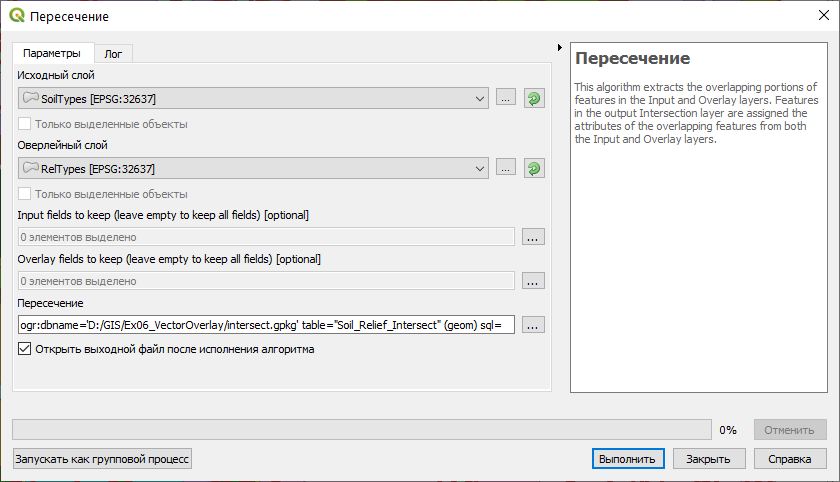
\includegraphics{images/Ex06/overlay2.png}
\item
  Нажмите «Выполнить», чтобы запустить вычисления.

  Результат вычислений добавится на карту и в таблицу слоёв под именем \texttt{Пересечение}.
\item
  Переименуйте добавленный слой в \texttt{Комбинации\ почвы-рельеф}.
\item
  Поместите полученный оверлеем слой между слоями типов почв и рельефа, и настройте его отображение в виде полигона без заливки с черной обводкой. Там, где границы совпадают с контурами типов рельефа, они будут черного цвета, а там где они совпадают с контурами типов почв, будет красная линия с черной обводкой.

  \includegraphics{images/Ex06/overlay3.png}
\item
  Раскройте атрибутивную таблицу слоя \emph{Комбинации почвы-рельеф}.
\end{enumerate}

\textbf{Вопрос 5}: Какие поля содержатся в атрибутивной таблице полученного слоя?

\hypertarget{overlay-merge}{%
\section{Слияние результатов пересечения с целью получения показателя пространственной связи}\label{overlay-merge}}

\protect\hyperlink{overlay}{В начало упражнения ⇡}

Поскольку каждый полигон в оверлейном слое содержит значение типа/подтипа почвы и типа рельефа, появляется возможность установить приуроченность типов и подтипов почв к определенным типам рельефа.

Чтобы подсчитать долю каждого типа рельефа в площади каждого подтипа почв, необходимо просуммировать площади каждой их уникальной комбинации. Например, дерново-карбонатные выщелоченные почвы (\emph{Д-в-к}) на крутых эрозионных склонах встречаются в пределах Сатинского полигона в виде 6 разрозненных участков, имеющих некоторую суммарную площадь. Эта площадь, деленная на суммарную площадь почв подтипа \emph{Д-в-к} даст вероятностный критерий приуроченности почв \emph{Д-в-к} к крутым эрозионным склонам. То же самое касается остальных комбинаций подтипов почв и типов рельефа.

С точки зрения рабочих процессов ГИС, операцию следует разбить на 5 шагов:

\begin{itemize}
\item
  подсчет суммарной площади каждой комбинации подтипа почв и типа рельефа;
\item
  подсчет суммарной площади каждого подтипа почв;
\item
  добавление поля, в которое будет записана процентная доля;
\item
  соединение таблиц комбинаций и подтипов почв по названию подтипа почв;
\item
  деление площади комбинации на площадь подтипа почв и запись результата в соответствующее поле.
\end{itemize}

\begin{quote}
Объединение разрозненных объектов, обладающих одинаковым набором атрибутов, осуществляется с помощью \emph{операции объединения по признаку} (Dissolve). Причем, если объекты примыкают друг к другу, граница между ними будет стерта, а если объекты разнесены в пространстве, на выходе получится составной объект (Multipart feature), состоящий из нескольких полигонов. Объединение по признаку --- это один из методов генерализации, он очень часто используется в геоинформационном анализе и картографировании.
\end{quote}

\begin{enumerate}
\def\labelenumi{\arabic{enumi}.}
\item
  Откройте инструмент геообработки «Объединение по признаку».
\item
  Выберите в качестве исходного слоя \emph{Комбинации почвы-рельеф}.
\item
  Нажмите на кнопку с изображением многоточия в строке \emph{Dissolve fields (optional)}, чтобы задать поля, по которым будет производиться слияние. В открывшемся списке отметьте поля \emph{SoilType}, \emph{SoilSubtype} и \emph{RelType}. Тем самым можно будет найти все уникальные комбинации подтипов почв и типов рельефа.

  \begin{quote}
  Поле \emph{SoilType} необходимо отметить для того, чтобы в таблице результирующего слоя сохранилась информация о типах почв. Это не повлияет на сам результат, поскольку количество комбинаций типа и подтипа почв равно количеству самих подтипов.
  \end{quote}
\item
  Укажите путь для сохранения результата объединения по признаку. Сохраните результат в тот же GeoPackage, что и результат пересечения, а слой назовите \texttt{Soil\_Relief\_Intersect\_Dissolve}.
\item
  Запустите выполнение инструмента.
\item
  После того, как результат появится в таблице содержания, закройте окно инструмента. Переименуйте полученный слой в \emph{Слияние комбинаций почвы-рельеф}.
\item
  Отключите этот слой в таблице содержания.
\end{enumerate}

\hypertarget{overlay-sumarea-subtypes}{%
\section{Объединение подтипов почв для подсчёта суммарной площади}\label{overlay-sumarea-subtypes}}

\protect\hyperlink{overlay}{В начало упражнения ⇡}

\begin{enumerate}
\def\labelenumi{\arabic{enumi}.}
\item
  Запустите инструмент объединения по признаку еще раз.
\item
  Выберите в качестве входных данных слой \emph{SoilTypes}.
\item
  В списке полей для объединения выберите поля \emph{SoilType} и \emph{SoilSubtype}.
\item
  Выходной набор данных сохраните в тот же GeoPackage с именем слоя \emph{SoilTypes\_Dissolve}.
\item
  Остальные параметры оставьте по умолчанию и запустите инструмент.
\item
  Назовите полученный слой \emph{Слияние подтипов почв}. В данном слое в результате операции слияния каждый подтип почв будет представлен единственным объектом.
\item
  Отключите этот слой в таблице содержания.
\end{enumerate}

\hypertarget{overlay-fieldcalc}{%
\section{Расчёт площадей объектов}\label{overlay-fieldcalc}}

\protect\hyperlink{overlay}{В начало упражнения ⇡}

В отличие от ArcGIS, QGIS не умеет автоматически пересчитывать площади объектов при изменении их геометрии. А изменения, которые мы произвели в процессе объединения по признаку, достаточно велики. Далее мы рассчитаем площади каждого объекта в «объединённых» слоях, затем выполним соединение атрибутивных таблиц и рассчитаем показатель связи на основе соотношения площадей.

\begin{enumerate}
\def\labelenumi{\arabic{enumi}.}
\item
  Откройте таблицу атрибутов слоя \emph{Слияние комбинаций почвы-рельеф}.
\item
  В заголовке таблицы найдите \textbf{Открыть калькулятор полей} (\includegraphics{images/Ex06/fieldcalc1.png}) или нажмите \texttt{Ctrl+I}.

  В QGIS, в отличие от ArcGIS и многих СУБД, не требуется отдельно создавать новое поле перед выполнением расчёта. Мы создадим новое поле, в котором будет записана площадь объекта в гектарах, и одновременно заполним его значениями с помощью калькулятора полей.
\item
  Введите имя поля \texttt{AREA\_HA\_INTERSECT} и установите тип данных «Десятичное число (real)».
\item
  Введите выражение \texttt{\$area\ /\ 10000} в поле «Выражение».

  \includegraphics{images/Ex06/fieldcalc2.png}

  Пояснение: \texttt{area()} --- системная функция QGIS, возвращающая площадь объекта. Значок \texttt{\$} означает, что функция будет применена к текущему объекту. Площадь вычисляется в единицах измерения площади, предусмотренных для системы координат источника данных. Для проецированных систем координат это, как правило, метры (реже футы). Назначение выражения \texttt{/\ 10000} постарайтесь определить самостоятельно.
\item
  Нажмите ОК. Слой перейдёт в режим редактирования, а в таблице атрибутов появится новый столбец.
\item
  Сохраните правки и выключите режим редактирования для слоя \emph{Слияние комбинаций почвы-рельеф}. Кнопка включения/выключения режима редактирования доступна не только в панели редактирования, но и в окне таблицы атрибутов.
\item
  Проделайте аналогичную операцию для слоя \emph{Слияние подтипов почв}. \textbf{Важно:} используйте другое имя для поля площади, например, \texttt{AREA\_HA\_SOILS}, чтобы избежать ошибки на следующем шаге.
\end{enumerate}

\hypertarget{overlay-join}{%
\section{Соединение таблиц по названию подтипа почв}\label{overlay-join}}

\protect\hyperlink{overlay}{В начало упражнения ⇡}

Для расчета пространственной взаимосвязи необходимо поделить площадь каждой комбинации на площадь соответствующего подтипа почв. Эти площади находятся сейчас в разных таблицах --- \emph{Слияние подтипов почв} и \emph{Слияние комбинаций почвы-рельеф}. Их можно соединить по полю подтипа почв.

\begin{quote}
\emph{Соединение таблиц} (table join) --- операция, в результате которой к одной таблице временно добавляются столбцы из другой таблицы. Чтобы установить соответствие между строками исходной и присоединяемой таблицы, необходимо иметь в каждой таблице поле с общими для них значениями. Например, это может быть числовой код объекта или, как в нашем случае, подтип почв (строковый тип данных).
\end{quote}

\begin{enumerate}
\def\labelenumi{\arabic{enumi}.}
\item
  Откройте свойства слоя \emph{Слияние комбинаций почвы-рельеф} и перейдите на вкладку \emph{Связи}.
\item
  Нажмите на кнопку с изображением знака «+» внизу, чтобы добавить новую связь.
\item
  Настройте параметры соединения, как показано на рисунке ниже:

  \includegraphics{images/Ex06/tablejoin1.png}

  \textbf{Вопрос 6}: Что такое «поле для объединения» и «целевое поле» в QGIS? К каким слоям относится каждое из них?
\item
  Примените изменения, закройте свойства слоя и откройте таблицу атрибутов.

  \textbf{Вопрос 7}: Что изменилось в таблице атрибутов после создания связи?
\end{enumerate}

\hypertarget{overlay-resulting}{%
\section{Вычисление результирующих значений показателя связи}\label{overlay-resulting}}

\protect\hyperlink{overlay}{В начало упражнения ⇡}

\begin{enumerate}
\def\labelenumi{\arabic{enumi}.}
\item
  Откройте таблицу атрибутов слоя \emph{Слияние комбинаций почвы-рельеф}, а затем вызовите калькулятор полей.
\item
  Укажите, что результат вычисления будет сохраняться в новое поле вещественного (real) типа, имя поля --- \texttt{Percent}
\item
  В окне ввода выражения составьте следующее выражение:

  \textbf{Площадь сочетания подтипа почв и типа рельефа / Площадь подтипа почв × 100 }

  \begin{quote}
  Подсказка: чтобы использовать значения полей в выражении, найдите в средней панели группу «Поля и значения». Добавляйте поля в выражение, кликая по их названиям дважды левой кнопкой мыши.
  \end{quote}
\item
  Запустите расчёт. После окончания расчёта посмотрите получившиеся значения в поле \emph{Percent}.
\item
  Удалите соединение таблиц через свойства слоя \emph{Слияние комбинаций почвы-рельеф} (вкладка «Связи», кнопка с изображением знака «минус» внизу).
\item
  Отсортируйте таблицу атрибутов по значению поля \emph{Percent} по убыванию. Выберите объекты, значение показателя связи для которых превышает 75 \%.
\item
  Скройте все столбцы, кроме типа почв, подтипа почв, типа рельефа и поля \emph{Percent.}. Для того, чтобы скрыть столбец в таблице атрибутов, нажмите на его название правой кнопкой мыши и выберите опцию \emph{Hide column}.
\item
  Скомпонуйте окно приложения так, чтобы было видно целиком карту, а также выделенные в таблице строки, а также столбцы, перечисленные в предыдущем пункте.

  \textbf{Скриншот 1:} окно карты и результирующая таблица

  \begin{quote}
  Примечание: если размер вашего экрана не позволяет скомпоновать окно QGIS в запрошенном виде, сделайте два скриншота: отдельно основное окно QGIS, отдельно таблицу атрибутов.
  \end{quote}
\item
  Сохраните документ карты.
\end{enumerate}

\hypertarget{appendix-ux441ux43fux440ux430ux432ux43eux447ux43dux44bux435-ux441ux432ux435ux434ux435ux43dux438ux44f}{%
\appendix}


\hypertarget{manual-catalog}{%
\chapter{Форматы пространственных данных}\label{manual-catalog}}

\hypertarget{ux448ux435ux439ux43f-ux444ux430ux439ux43bux44b}{%
\section{Шейп-файлы}\label{ux448ux435ux439ux43f-ux444ux430ux439ux43bux44b}}

\hypertarget{geopackage}{%
\section{GeoPackage}\label{geopackage}}

\hypertarget{ux431ux430ux437ux44b-ux433ux435ux43eux434ux430ux43dux43dux44bux445-esri}{%
\section{Базы геоданных ESRI}\label{ux431ux430ux437ux44b-ux433ux435ux43eux434ux430ux43dux43dux44bux445-esri}}

  \bibliography{book.bib,packages.bib}

\end{document}
